%%================================================
%% Chapter 4
%%================================================
\chapter{ผลการดำเนินงานและอภิปรายผล}
%\label{result}
\label{chapter4}
\section{Use Case Diagram ของ Website}
\begin{figure}[H]
    \captionsetup{justification=centering}
    \centering
    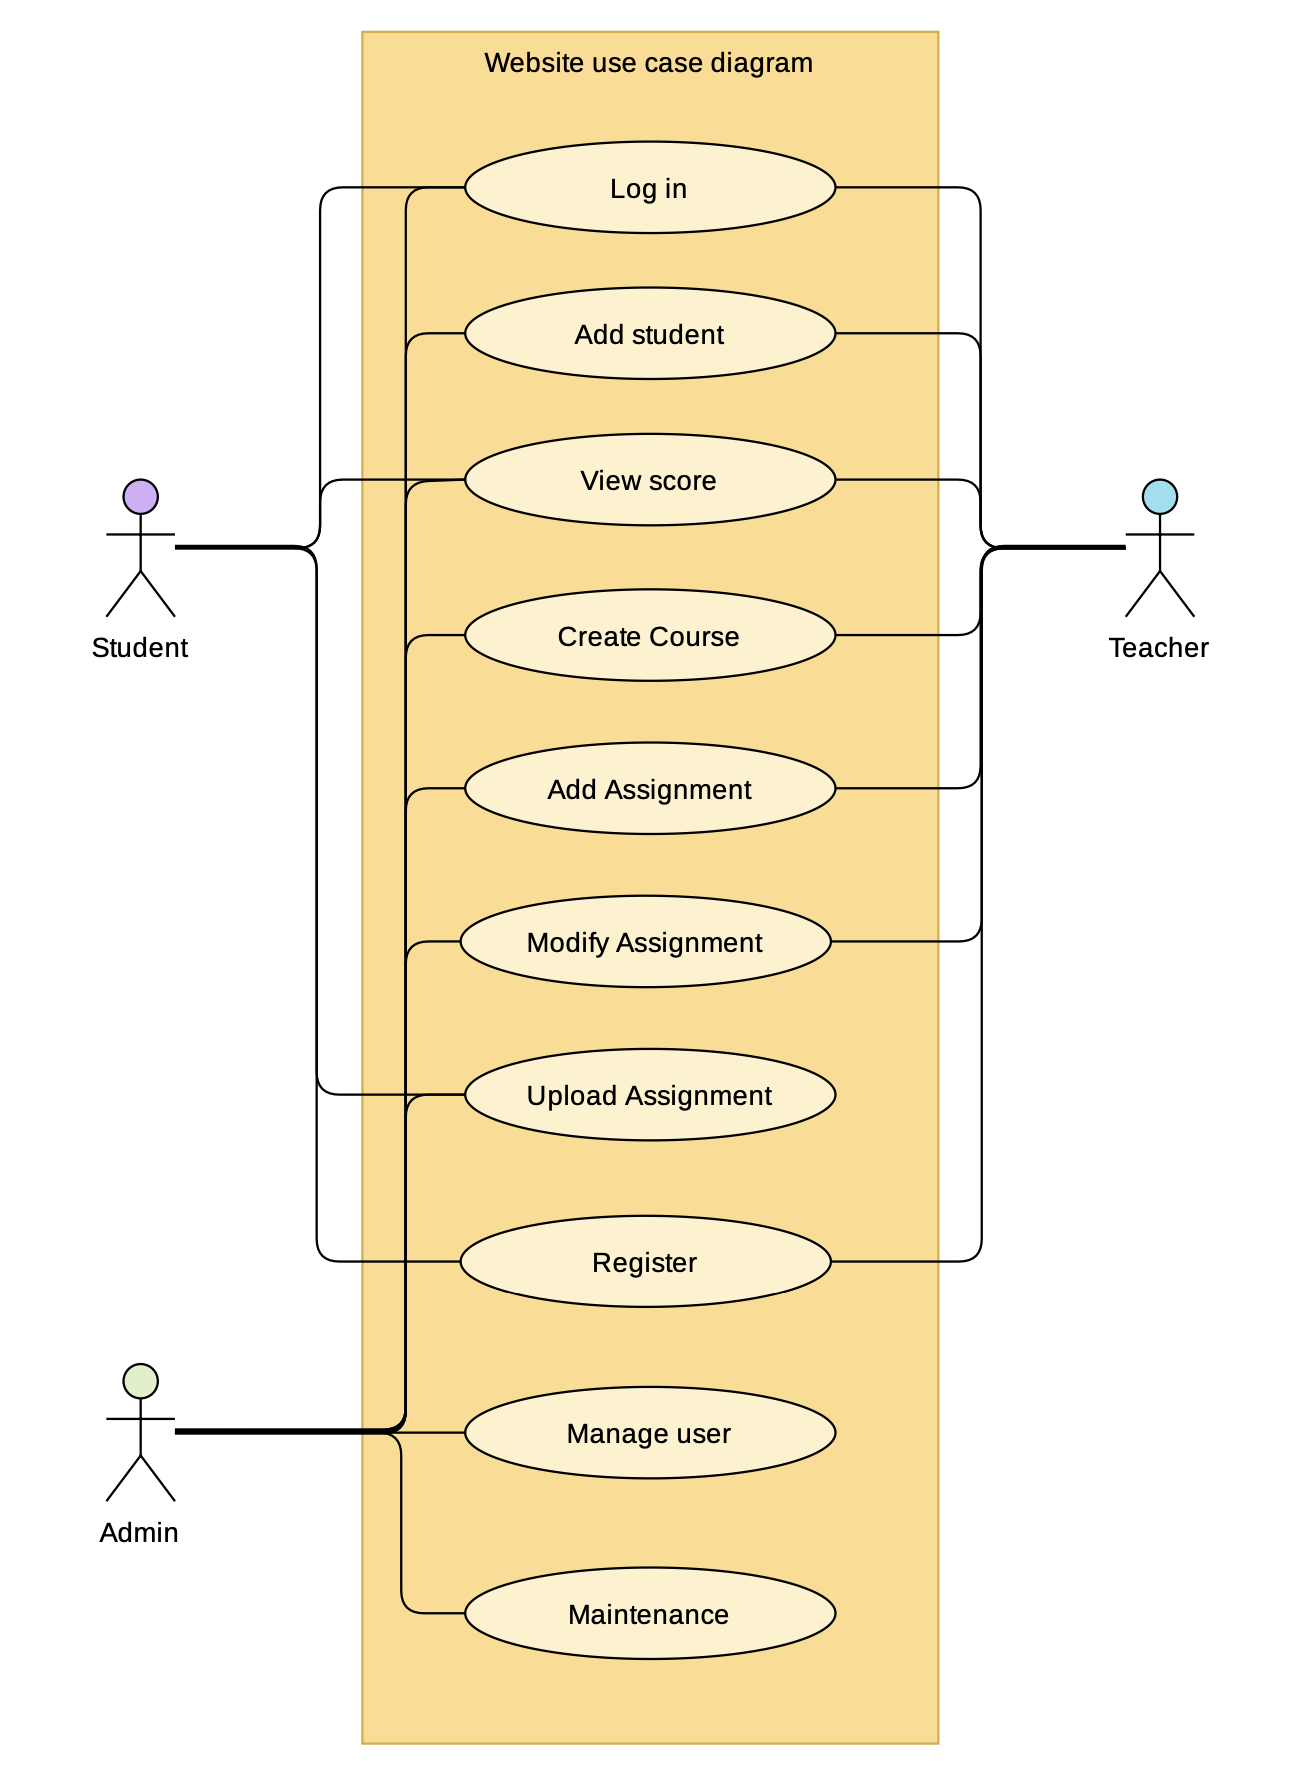
\includegraphics[width=5.5in]{figures/chapter4/usecase.png}
    \caption{แสดงสิทธิการใช้งานของ Student, Teacher และ Admin}
    \label{figure:usecase}
\end{figure}
\newpage
\noindent จากรูปที่ี่ \ref{figure:usecase} แสดงให้เห็นถึงสิทธิการเข้าถึงของแต่ละบุคคลในการใช้งาน Website โดยมีดังนี้
\begin{itemize}
    \item Admin สามารถเข้าถึงและจัดการ Website ได้ทุกส่วน ร่วมไปถึงการจัดการ User และ ดูแลระบบ
    \item Teacher สามารถเข้าถึง Website ได้ทุกส่วน สามารถสร้างและแก้ไข Course, Assignment และ คะแนนของ Student ทุกคน
    \item Student สามารถเข้าถึงหน้า Website ได้แค่บางส่วนเท่านั้น โดยสามารถดูหน้า Homepage,  Profile, Course ที่ลงเรียน, Assignment ของ Course นั้น และ ดูคะแนนของตนเอง
\end{itemize}

\section{การทำงานของ Website จริง}
จากที่ได้ทำการตั้งค่าและออกแบบ UI ของ Website แล้วนำมาเขียนโปรแกรมเพื่อใช้งานจริง จะได้รูปแบบของ Website ที่แบ่งออกเป็น 3 ส่วน ดังนี้

\subsection{ส่วนของ Admin หรือ ผู้ดูแลระบบ}
Admin หรือ ผู้ดูแลระบบสามารถทำการจัดการ แก้ไข และดูแลระบบในส่วนหลังบ้านได้ดังรูปต่อไปนี้
\begin{figure}[H]
    \captionsetup{justification=centering}
    \centering
    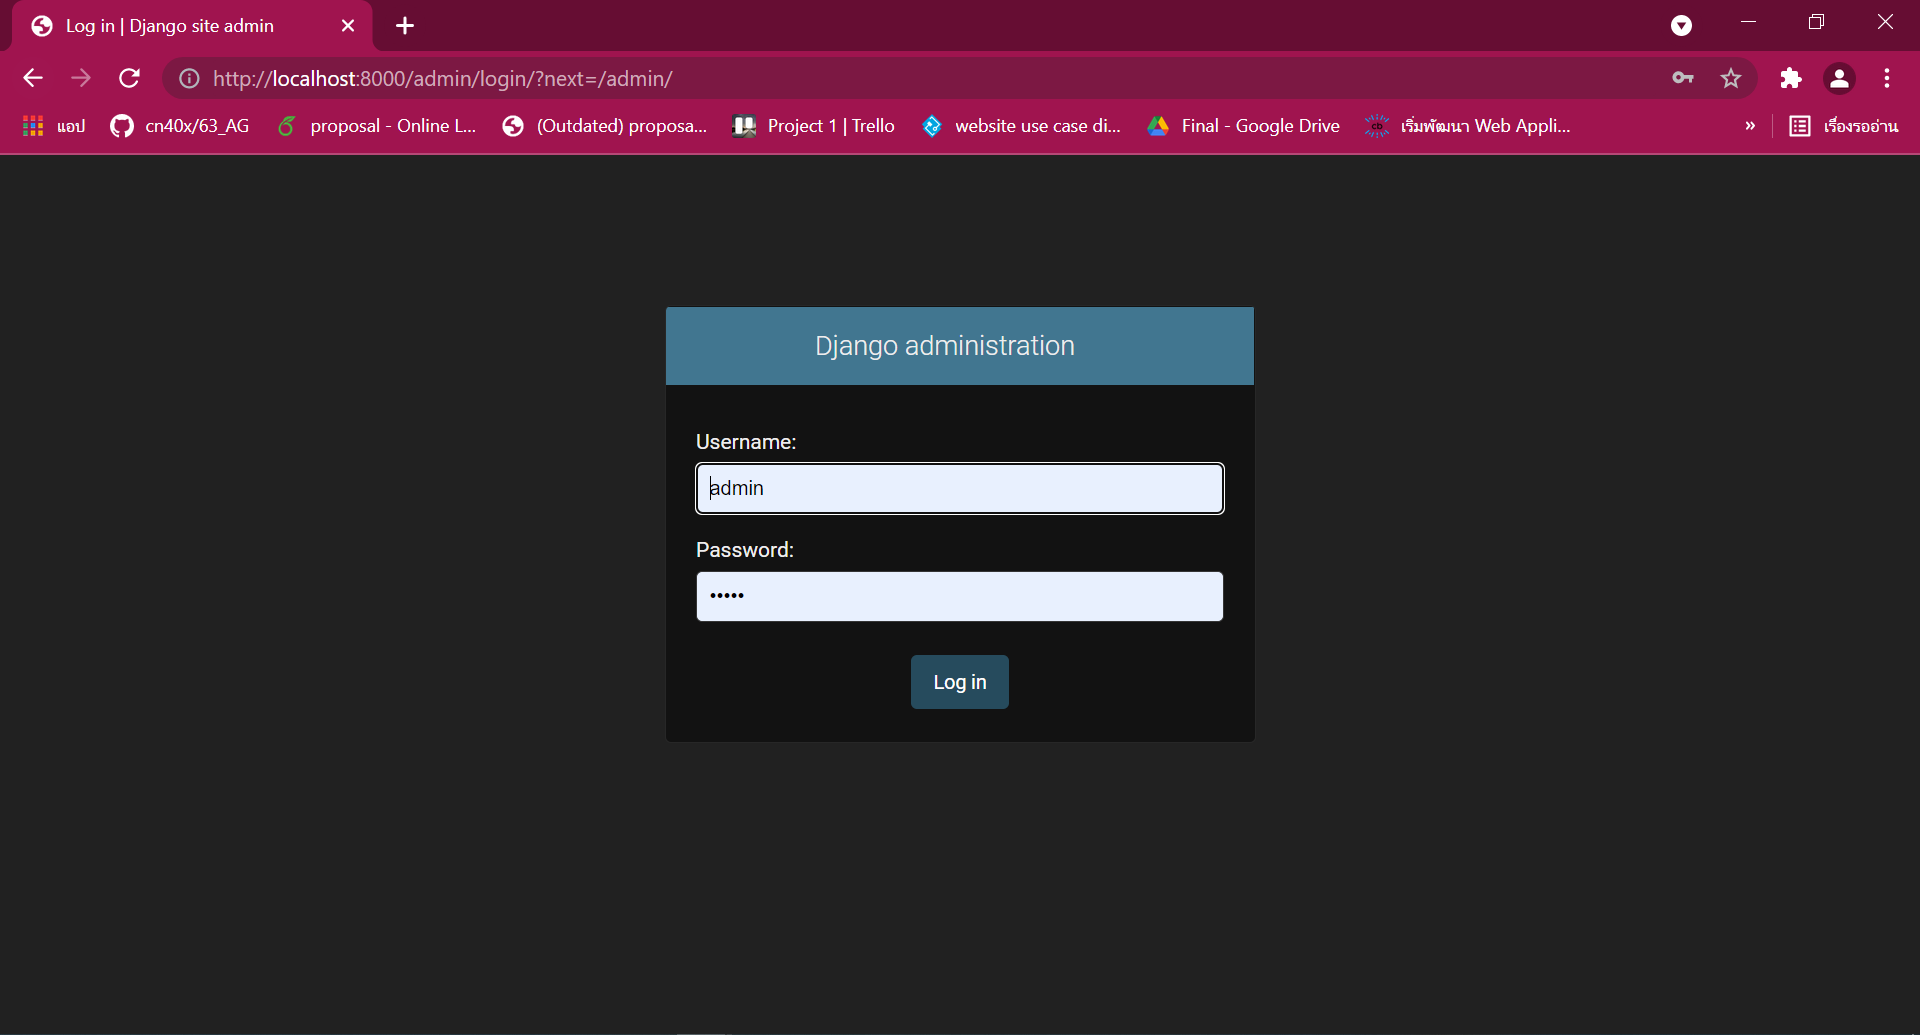
\includegraphics[width=5in]{figures/admin.png}
    \caption{การ log in เข้าใช้งานของ Admin}
    \label{figure:adminsite}
\end{figure}

\begin{figure}[!thb]
    \captionsetup{justification=centering}
    \centering
    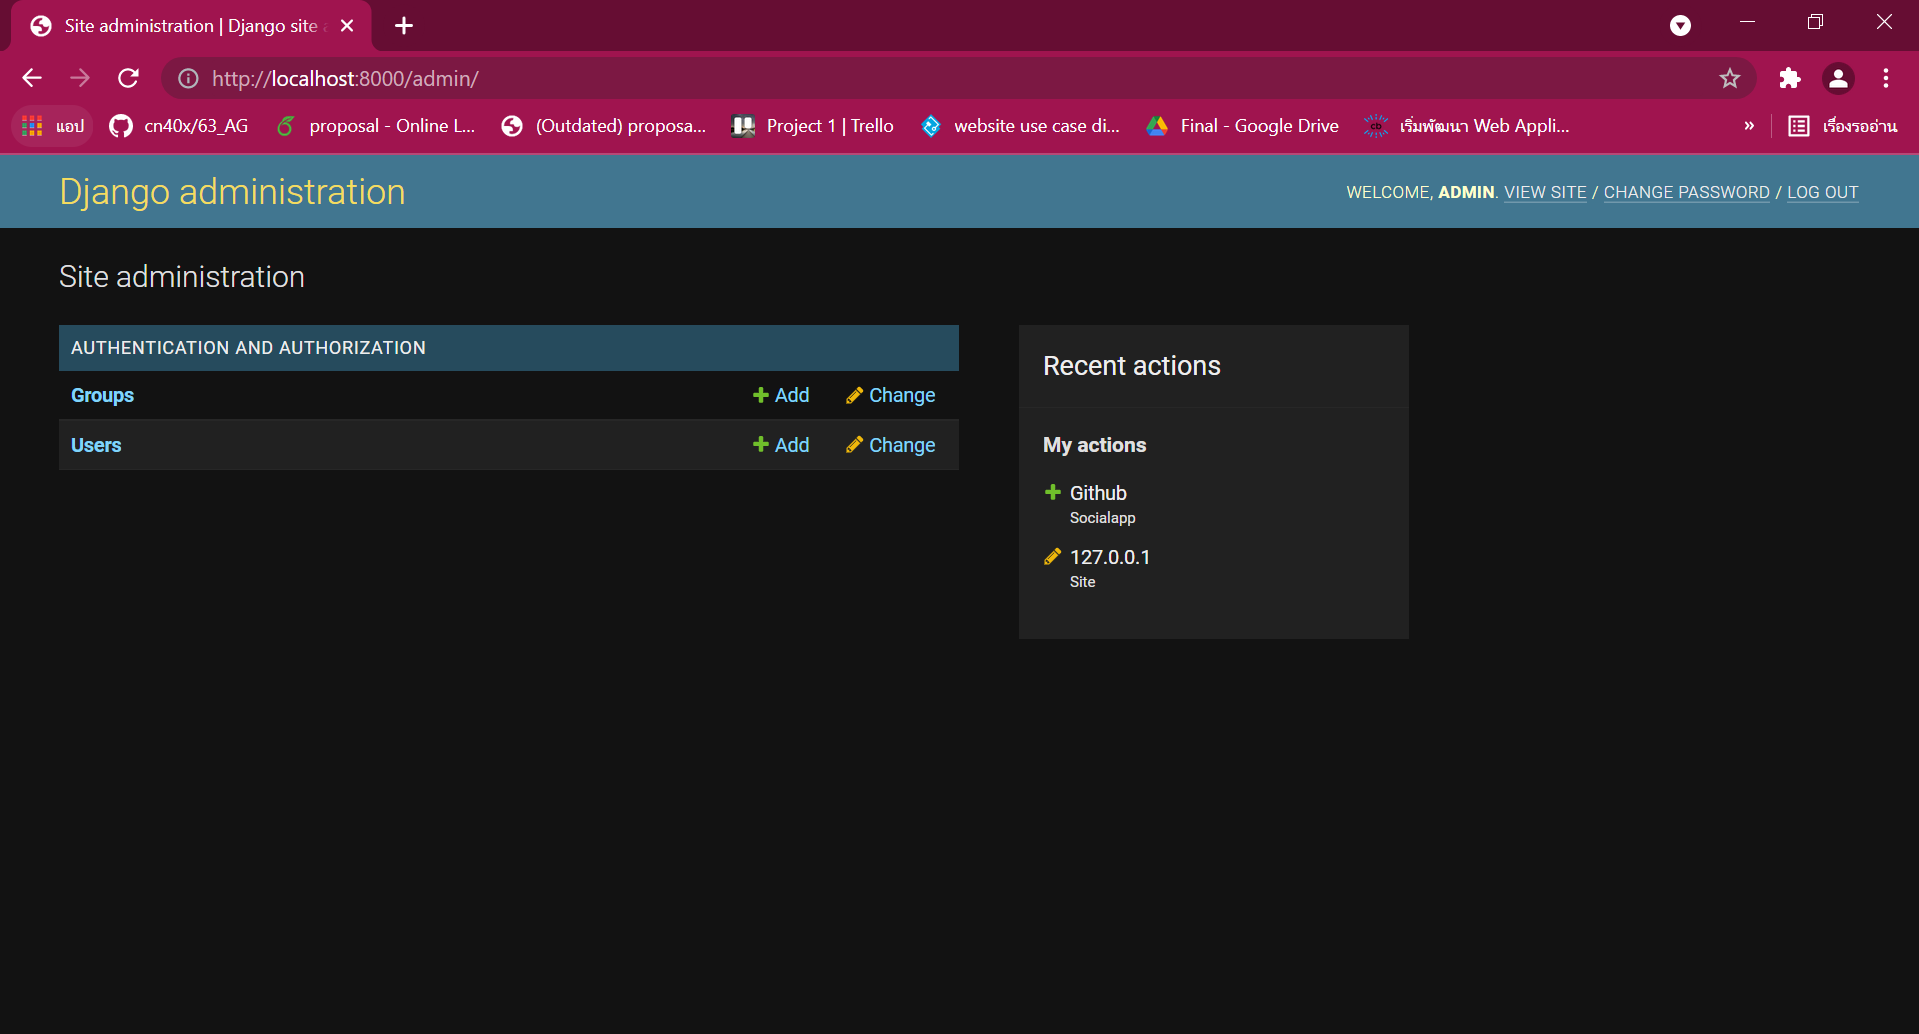
\includegraphics[width=5in]{figures/adminlogin.png}
    \caption{การดูแล Website ผ่านระบบหลังบ้าน}
    \label{figure:adminsite}
\end{figure}

\subsection{ส่วนของ Teacher หรือ ผู้สอน}

\begin{figure}[H]
    \captionsetup{justification=centering}
    \centering
    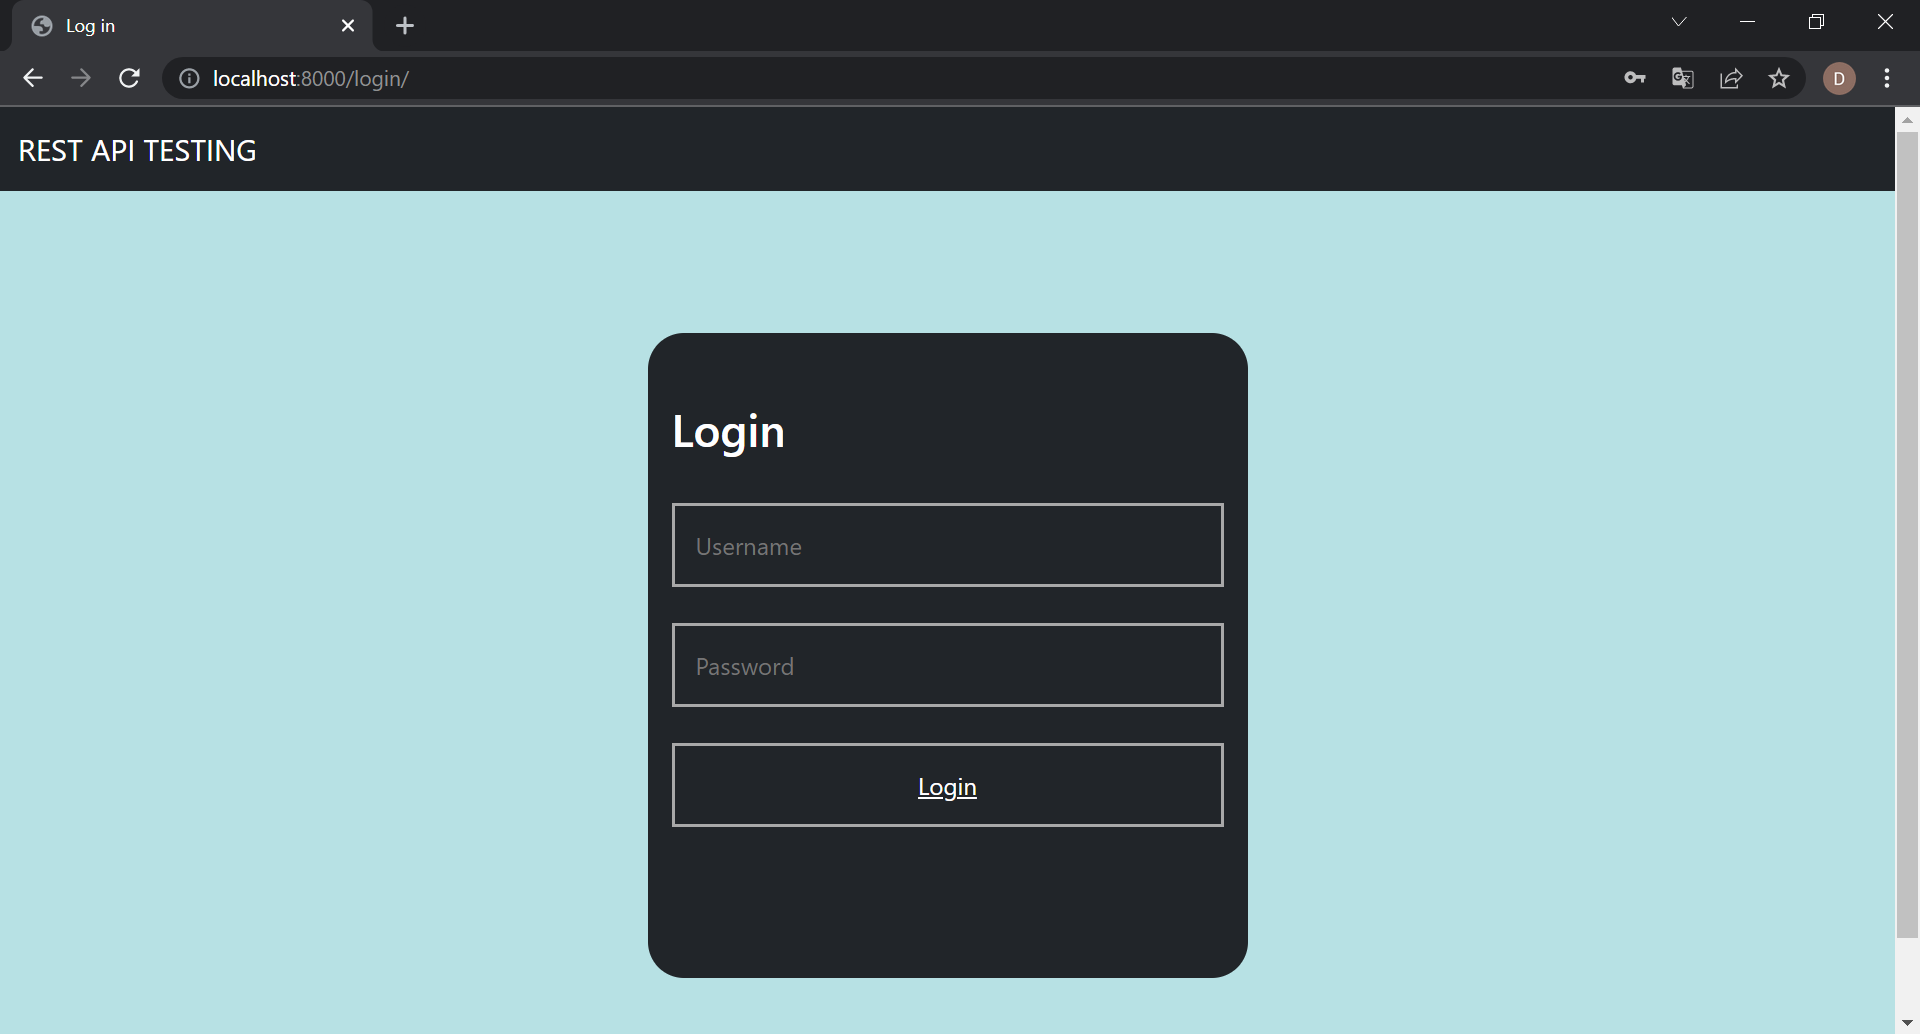
\includegraphics[width=5in]{figures/chapter4/login.PNG}
    \caption{หน้า Log in ฝั่ง Teacher}
    \label{figure:login}
\end{figure}
เริ่มจาก Teacher ทำการ Log in ด้วย Username และ Password ของตนเองที่ถูกกำหนดสิทธิไว้่ให้สามารถเข้าถึงทุกส่วนของหน้า Website ได้ ซึ่งหลังจากทำการ Log in เรียบร้อยแล้ว จะเข้ามายังหน้าของ Homepage ซึ่งเป็นหน้าแรกหลังจากทำการ Log in เรียบร้อยแล้ว
\newpage

\begin{figure}[H]
    \captionsetup{justification=centering}
    \centering
    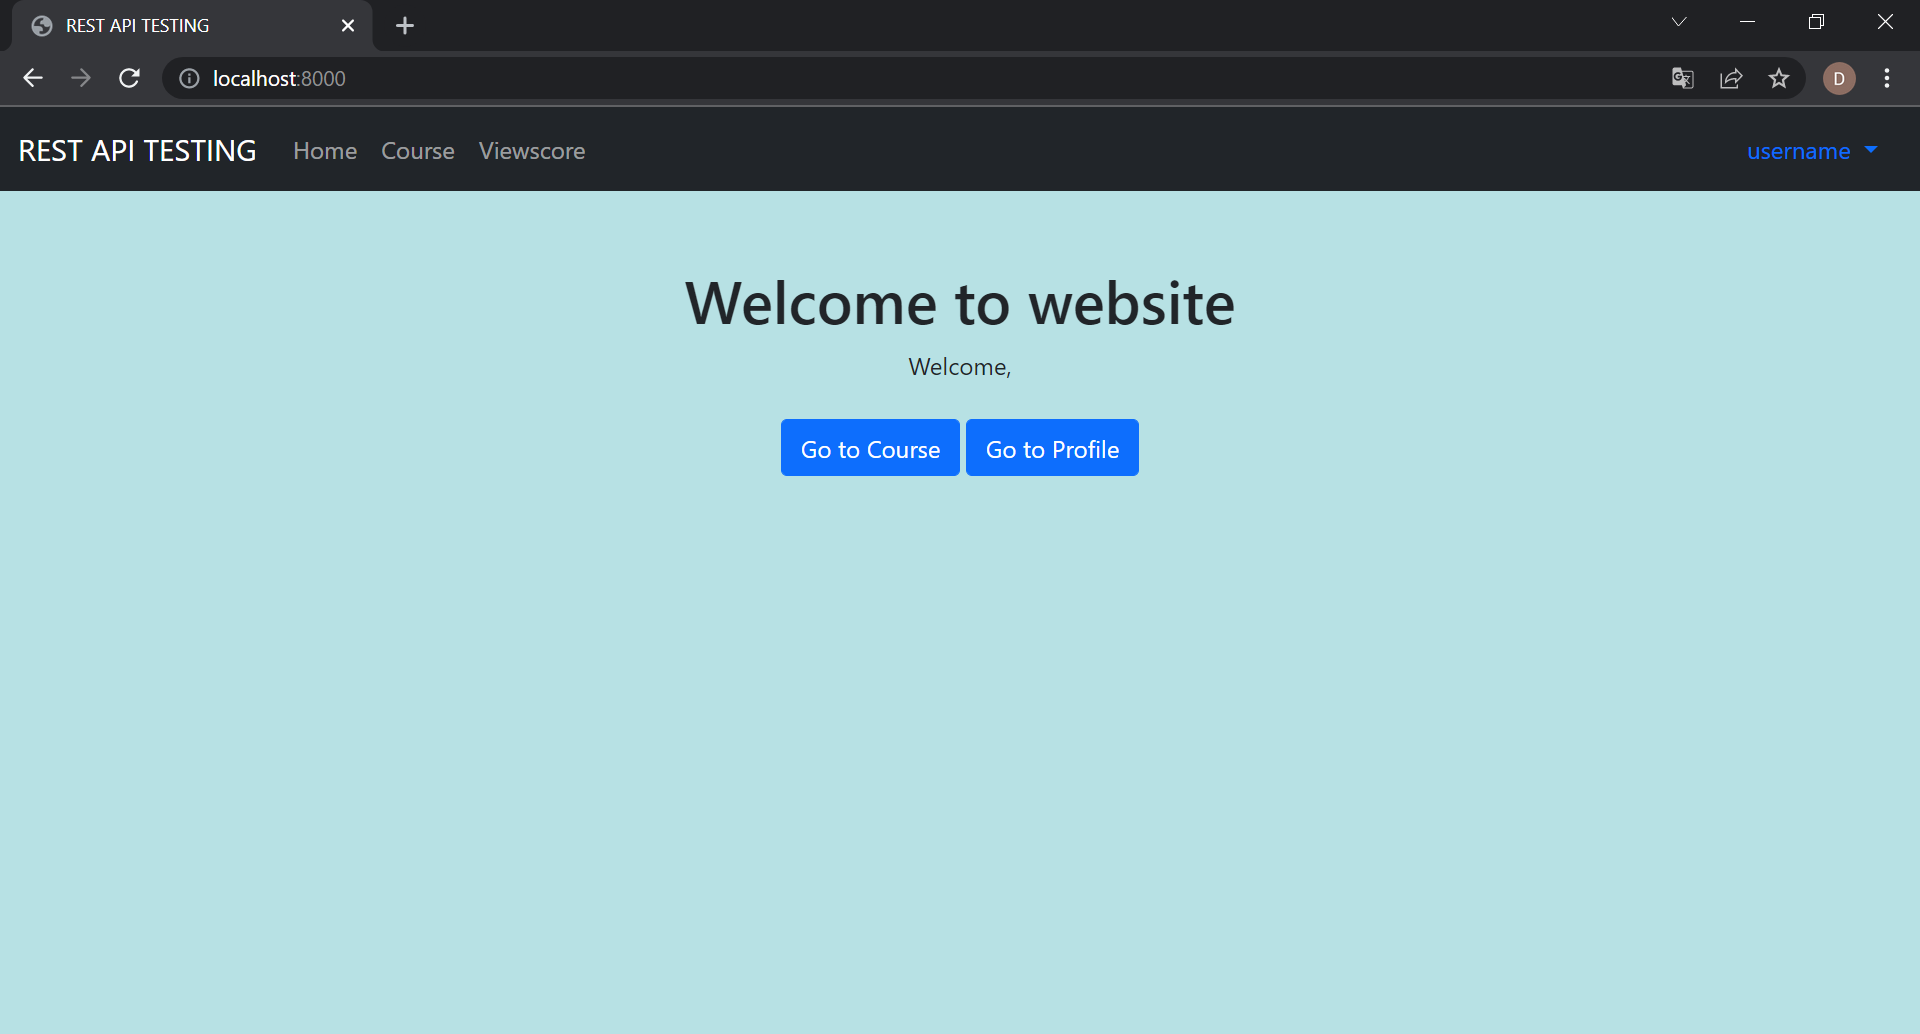
\includegraphics[width=5in]{figures/chapter4/homepage.PNG}
    \caption{หน้า Homepage ฝั่ง Teacher}
    \label{figure:homepage}
\end{figure}
สังเกตว่าหน้า Homepage Teacher สามารถเข้าไปยังหน้าต่าง ๆ ของ Website ผ่านหน้าหลักนี้ ซึ่งจะแสดงเมนูต่าง ๆ ที่สามารถเข้าถึงได้

\begin{figure}[H]
    \captionsetup{justification=centering}
    \centering
    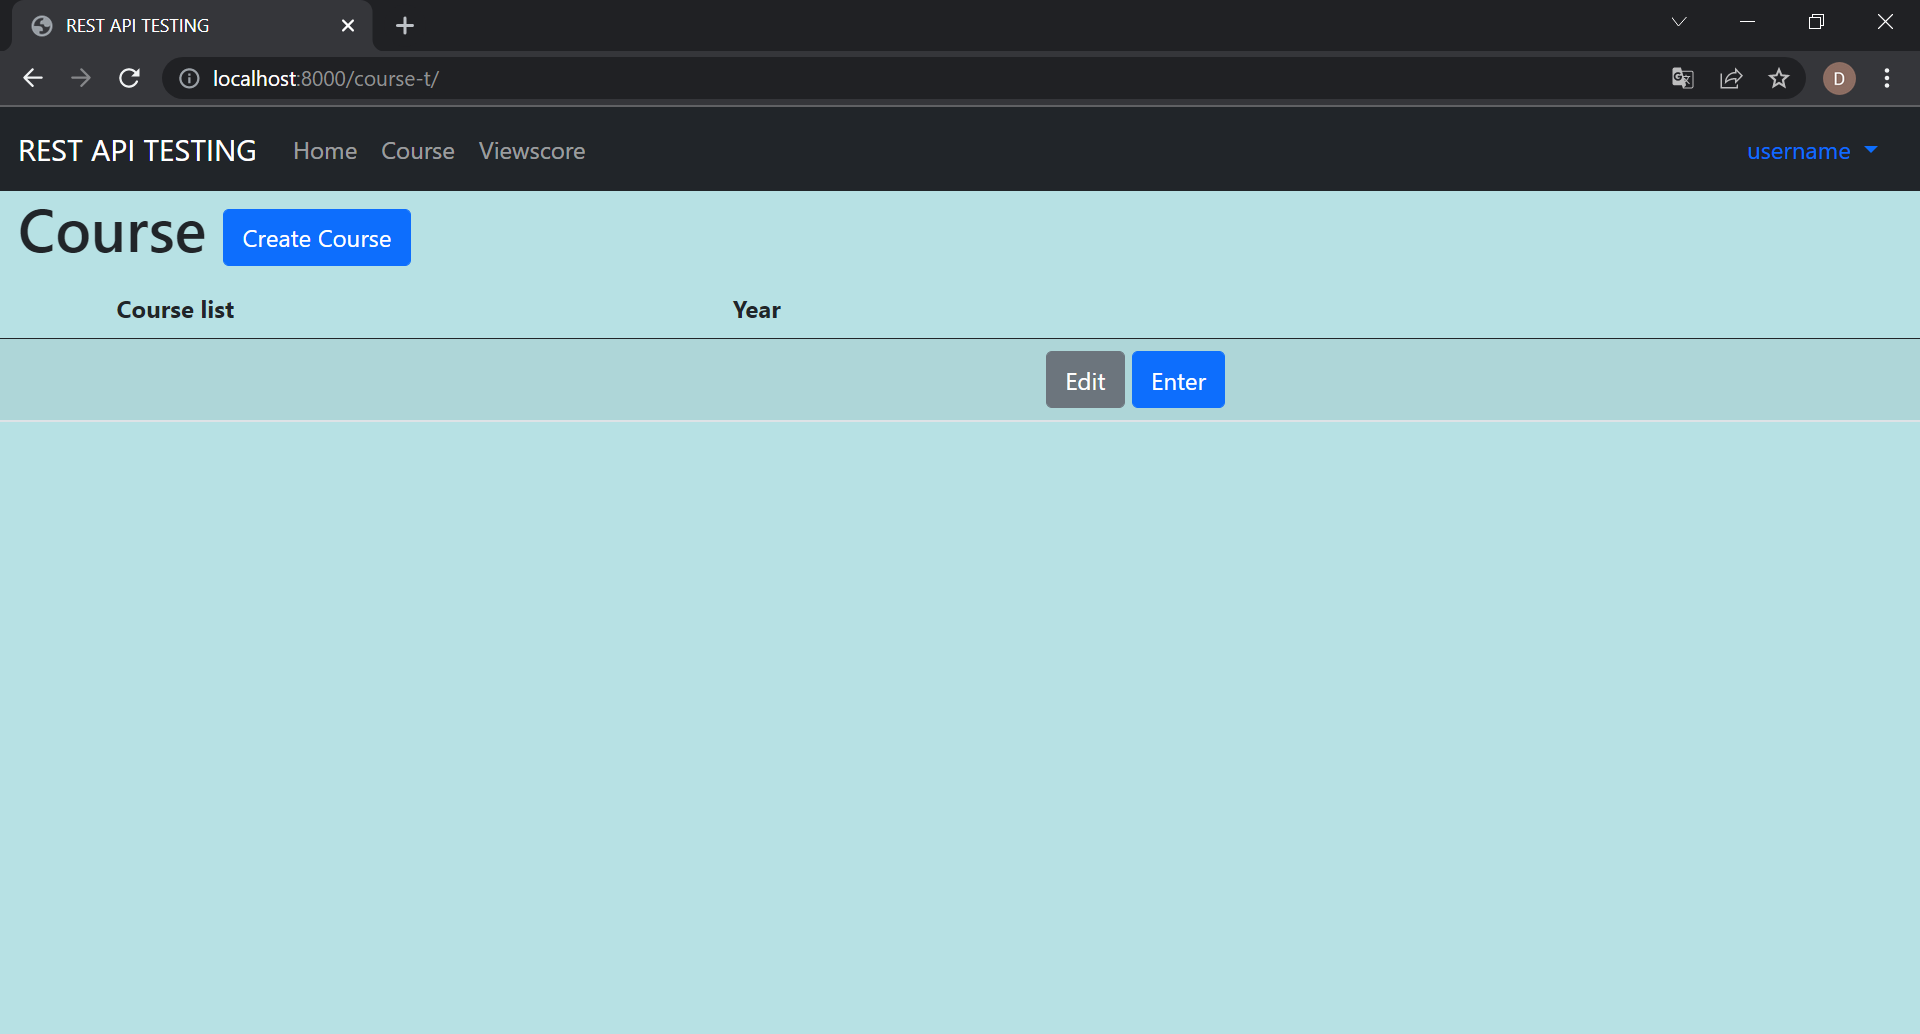
\includegraphics[width=5in]{figures/chapter4/courseteacher.PNG}
    \caption{หน้า Course ฝั่ง Teacher}
    \label{figure:course}
\end{figure}
เมื่อทำการกดปุ่ม Go to Course จะสามารถเข้าไปยังหน้า Course ซึ่งแสดงรายวิชาที่มีอยู่บน Website โดย Teacher สามารถเพิ่มรายวิชาได้โดยการกดปุ่ม Create Course เพื่อทำการสร้างวิชาใหม่ขึ้นมา
\newpage

\begin{figure}[H]
    \captionsetup{justification=centering}
    \centering
    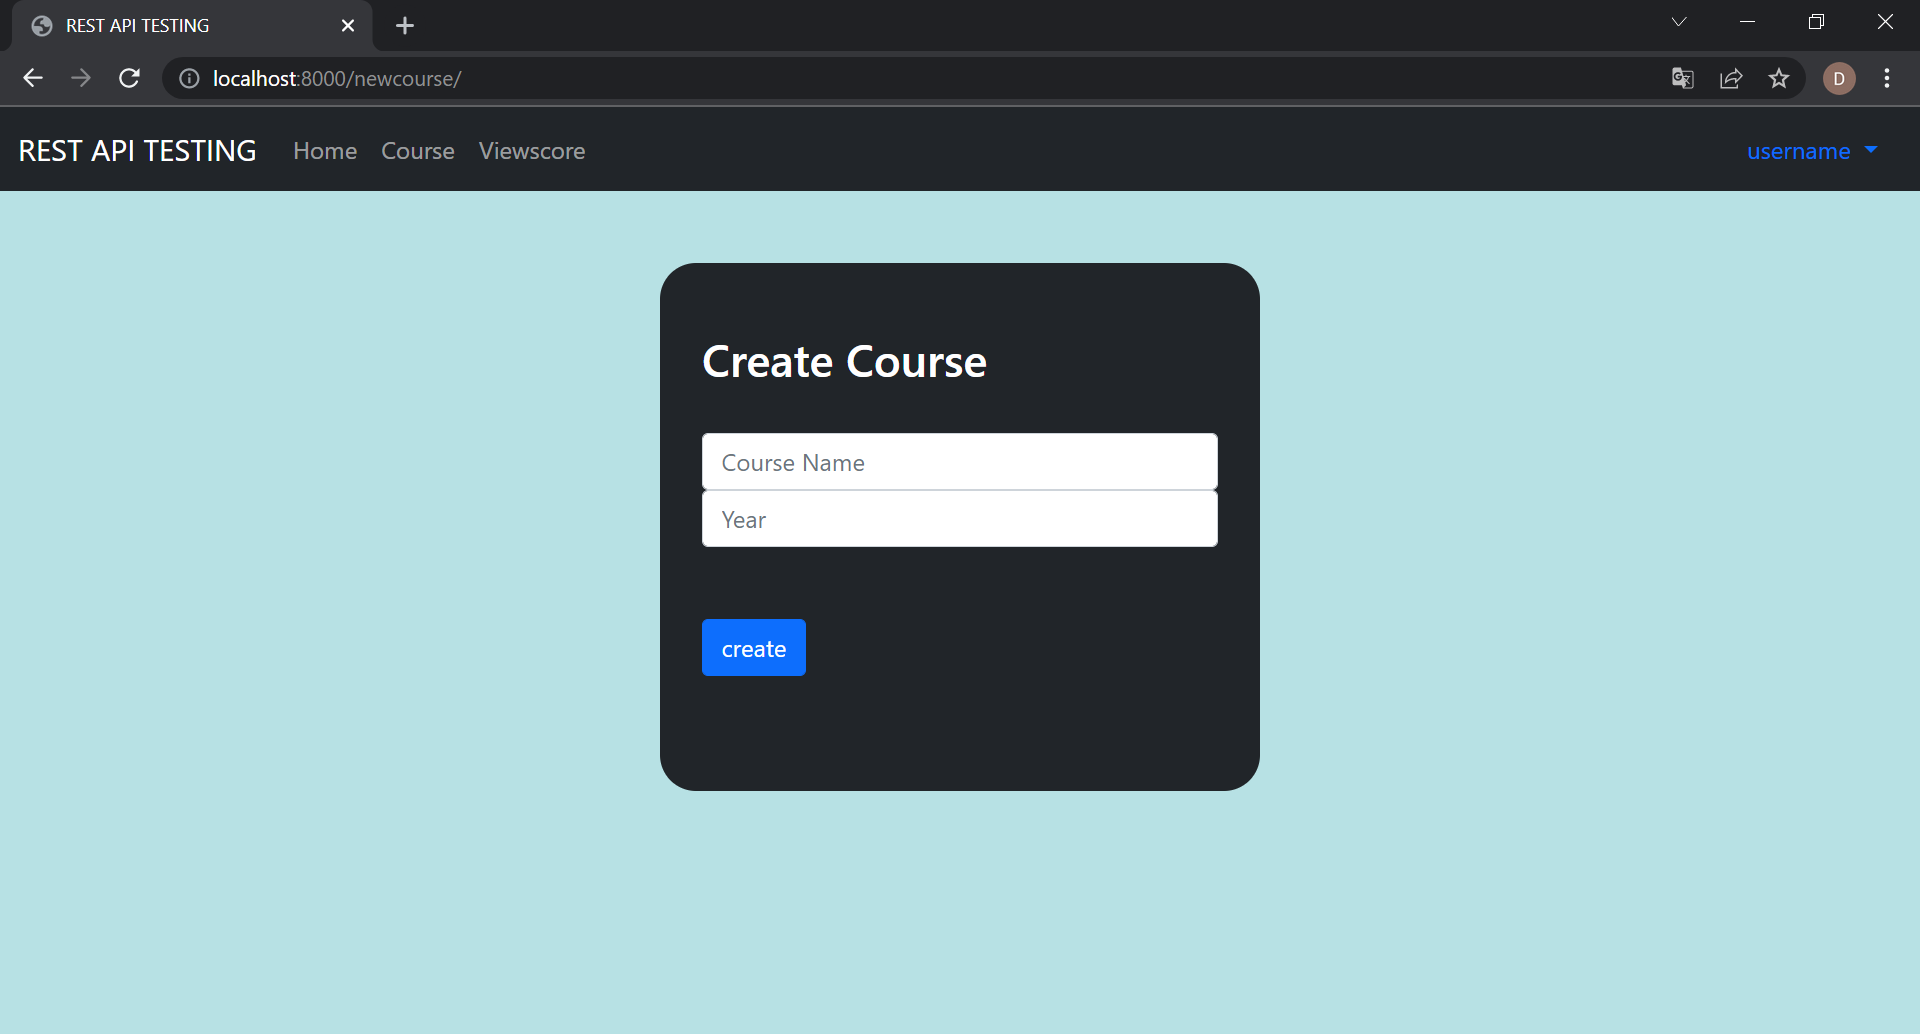
\includegraphics[width=5in]{figures/chapter4/createcourse.PNG}
    \caption{หน้า Create Course สำหรับ Teacher}
    \label{figure:createcourse}
\end{figure}
เมื่อ Teacher กดปุ่ม Create Course เข้ามาแล้วจะพบกับหน้าดังรูป \ref{figure:createcourse} จากนั้นจะมีกล่องข้อความให้ Teacher สามารถกรอกชื่อวิชา และ ปีการศึกษานั้น จากนั้นทำการกดปุ่ม Create

\begin{figure}[H]
    \captionsetup{justification=centering}
    \centering
    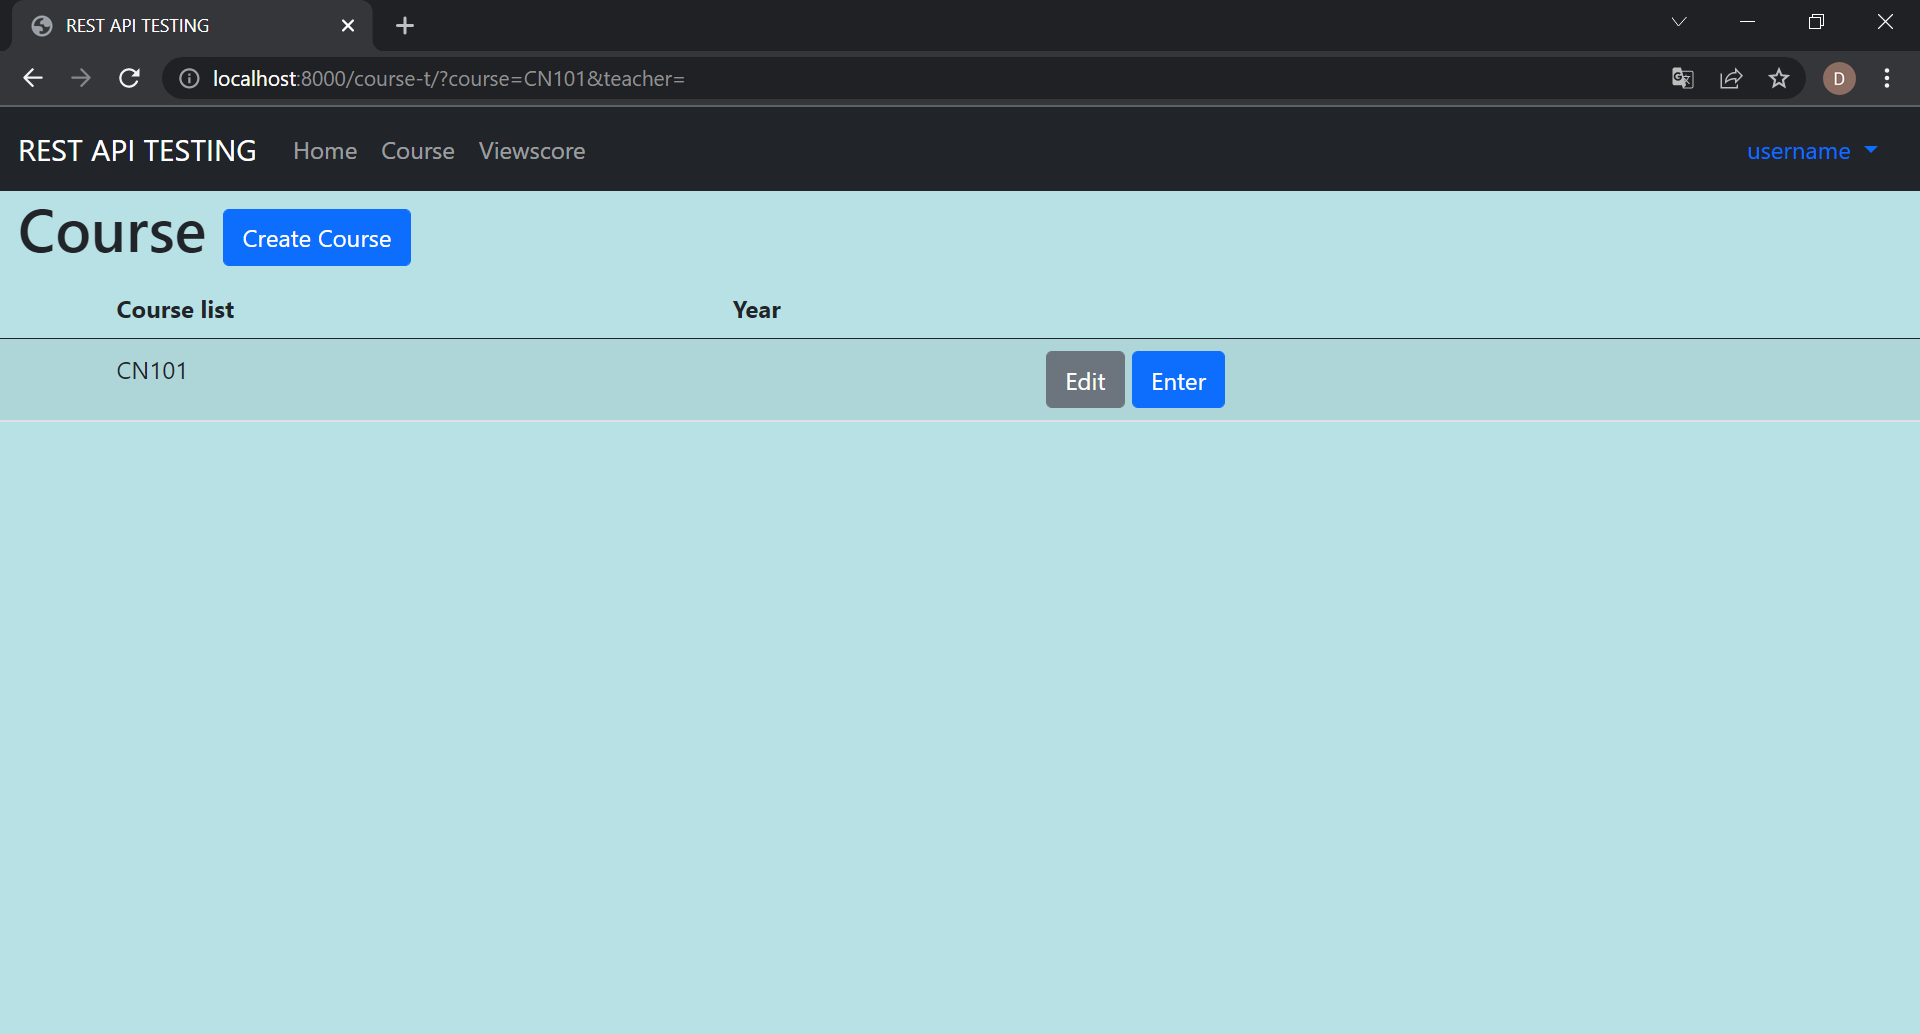
\includegraphics[width=5in]{figures/chapter4/cn101.PNG}
    \caption{แสดงรายชื่อวิชาหลังจากสร้างเสร็จ}
    \label{figure:course2}
\end{figure}
จะสังเกตได้่ว่าเมื่อทำการกดปุ่ม Create แล้วจากรูป \ref{figure:createcourse} จะมีชื่อวิชาแสดงขึ้นมาบนหน้า Course จากนั้นเมื่อต้องการเข้าไปยังหน้า Assignment ของวิชานี้ สามารถทำได้โดยการกดปุ่ม Enter ซึ่งหาก Teacher ต้องการลบหรือแก้ไขวิชานี้ สามารถทำได้โดยการกดปุ่ม Edit 
\newpage

\begin{figure}[H]
    \captionsetup{justification=centering}
    \centering
    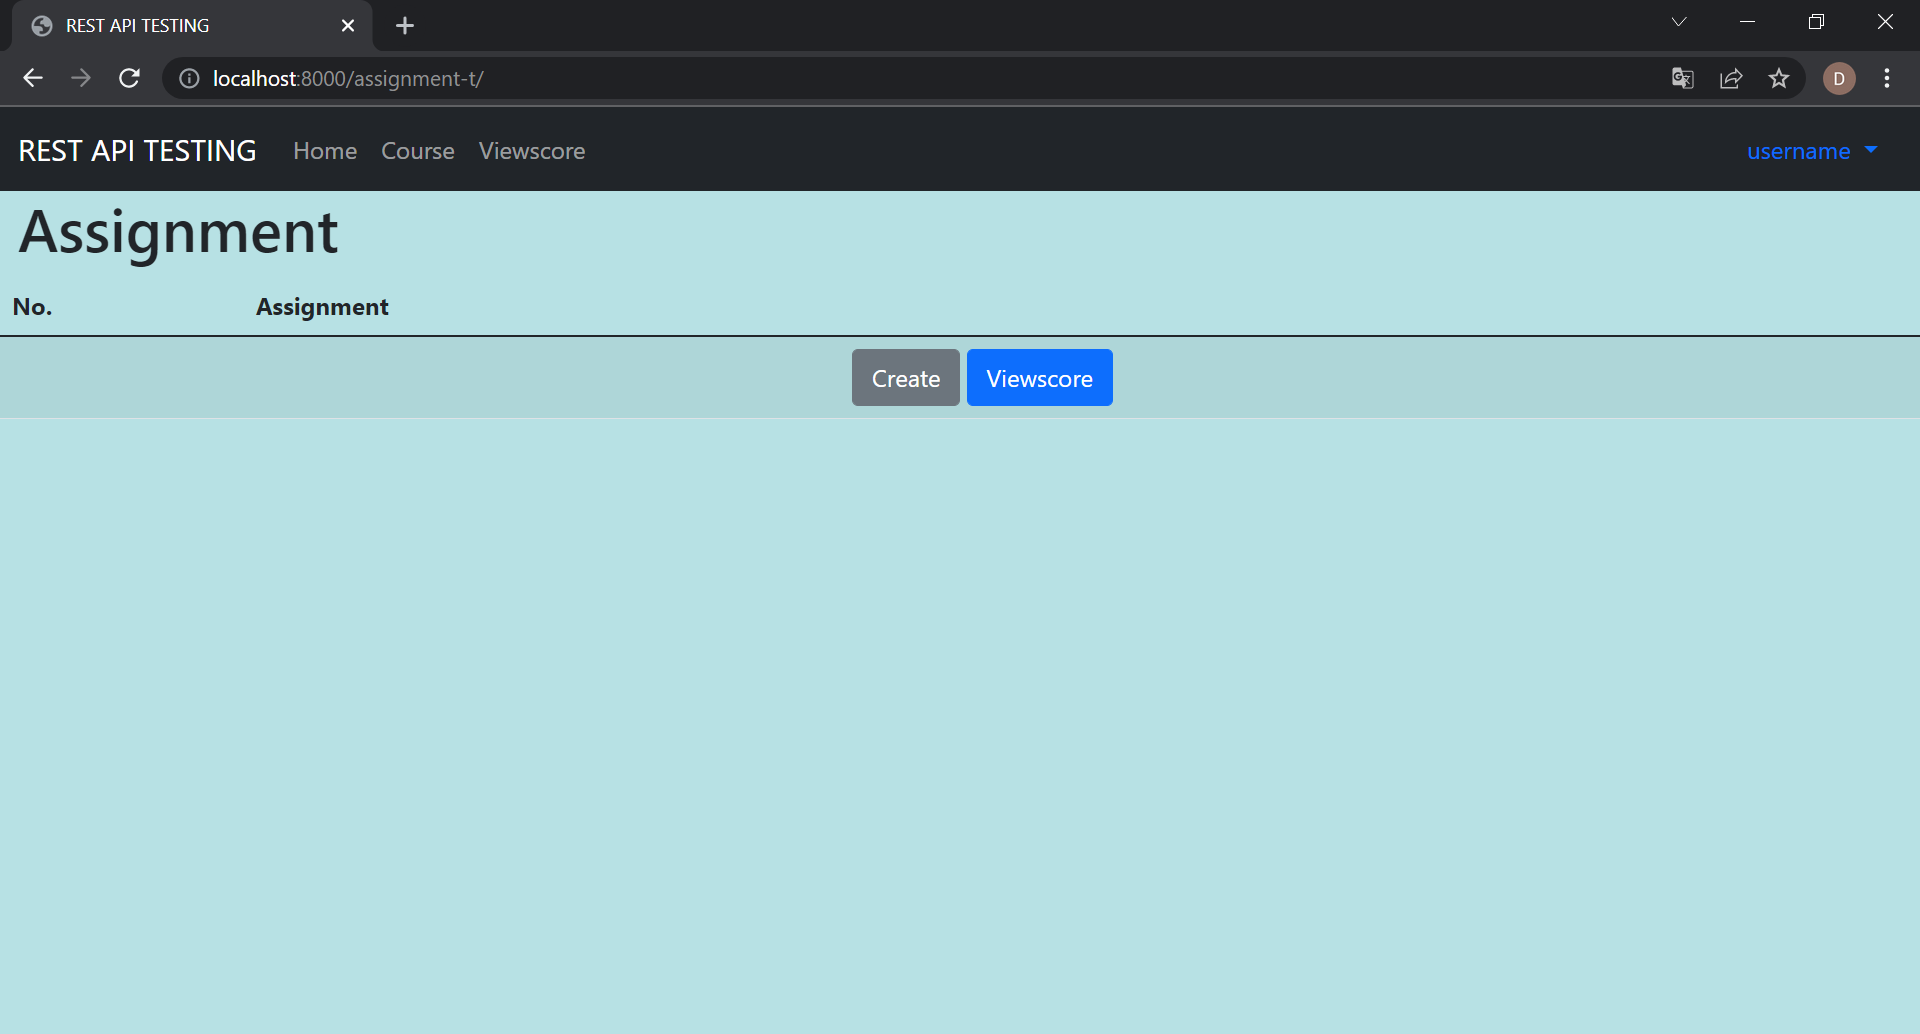
\includegraphics[width=5in]{figures/chapter4/assignteacher.PNG}
    \caption{หน้า Assignment ฝั่ง Teacher}
    \label{figure:assign}
\end{figure}
เมื่อเข้ามาในหน้าของ Assignment จะแสดงงานของวิชานั้น หาก Teacher ต้องการสร้าง Assignment ใหม่ขึ้นมา สามารถทำได้โดยการกดปุ่ม Create

\begin{figure}[H]
    \captionsetup{justification=centering}
    \centering
    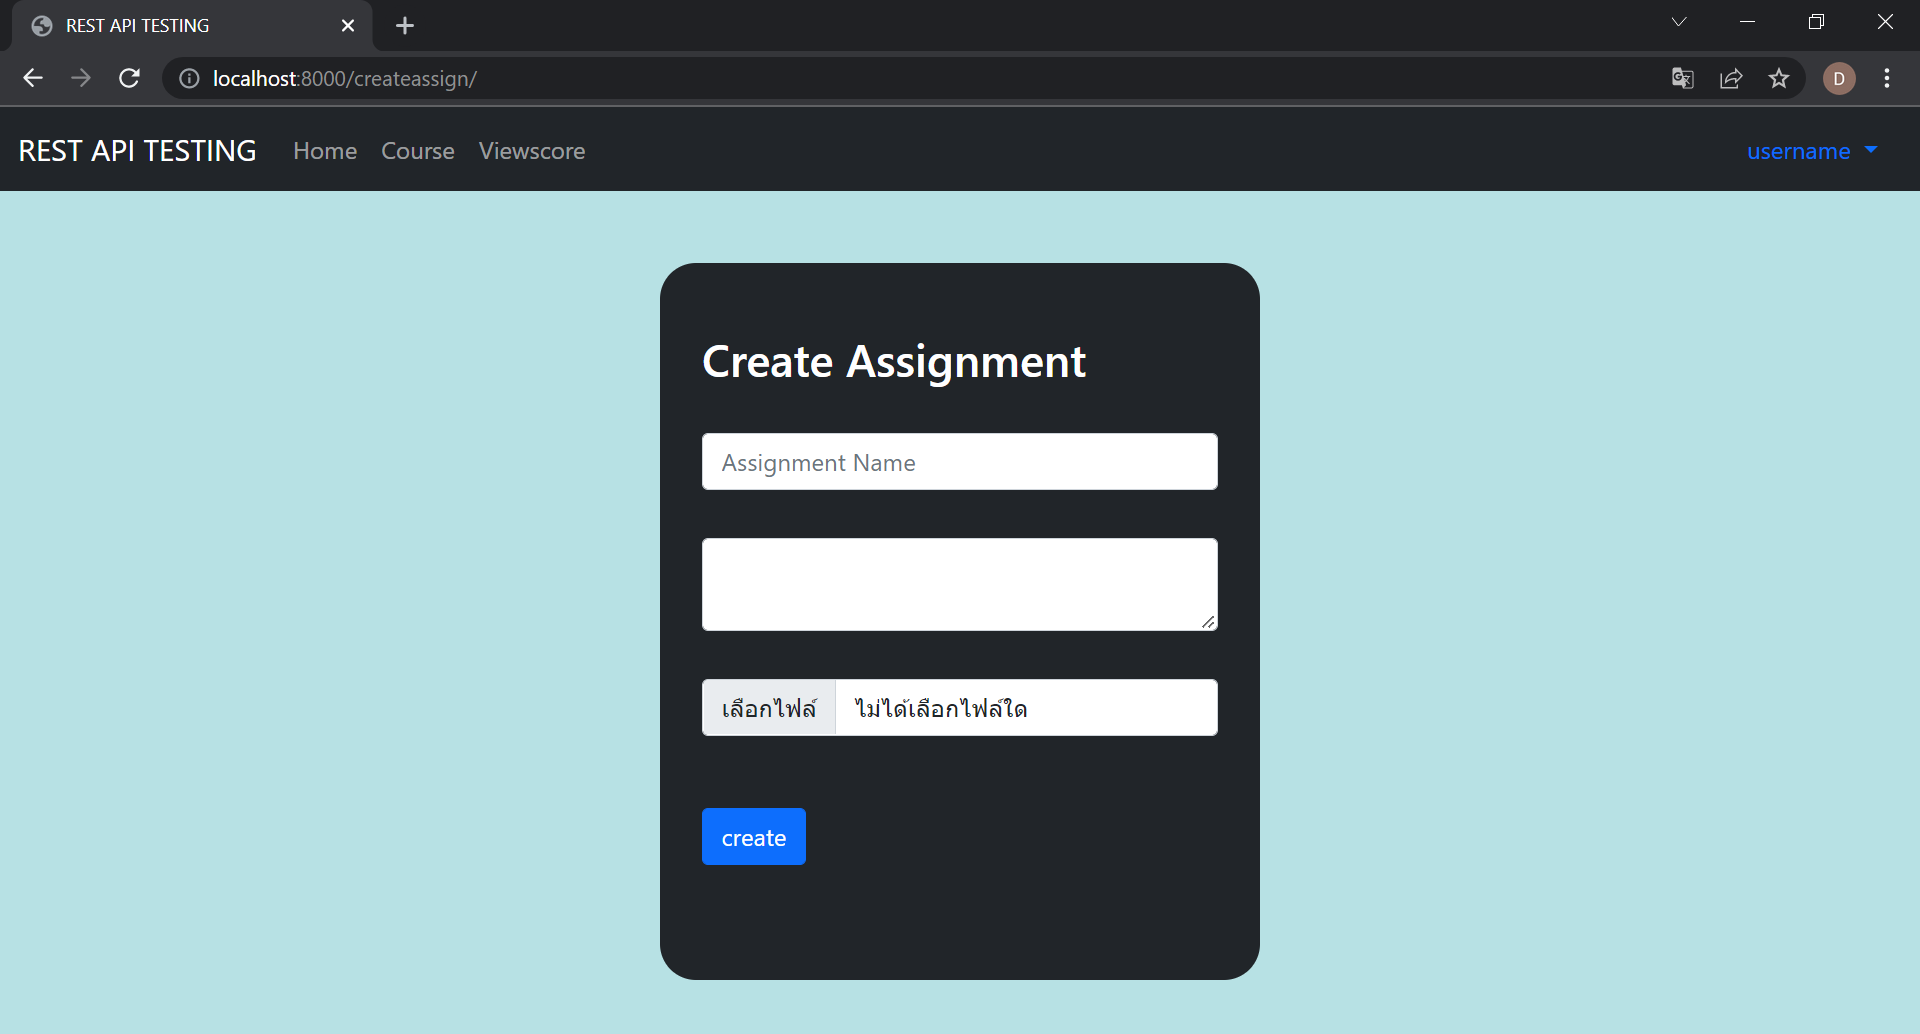
\includegraphics[width=5in]{figures/chapter4/createassign.PNG}
    \caption{หน้า Create Assignment สำหรับ Teacher}
    \label{figure:createassign}
\end{figure}
เมื่อเข้ามาในหน้าของ Create Assignment จะสังเกตว่ามีกล่องข้อความให้ Teacher \mbox{สามารถ}กำหนดชื่อ Assignment สามารถเพิ่มคำอธิบาย และ สามารถแนบไฟล์สำหรับ Assignment นี้ เข้าไปได้ จากนั้นทำการกดปุ่ม Create เพื่อสร้าง
\newpage

\begin{figure}[H]
    \captionsetup{justification=centering}
    \centering
    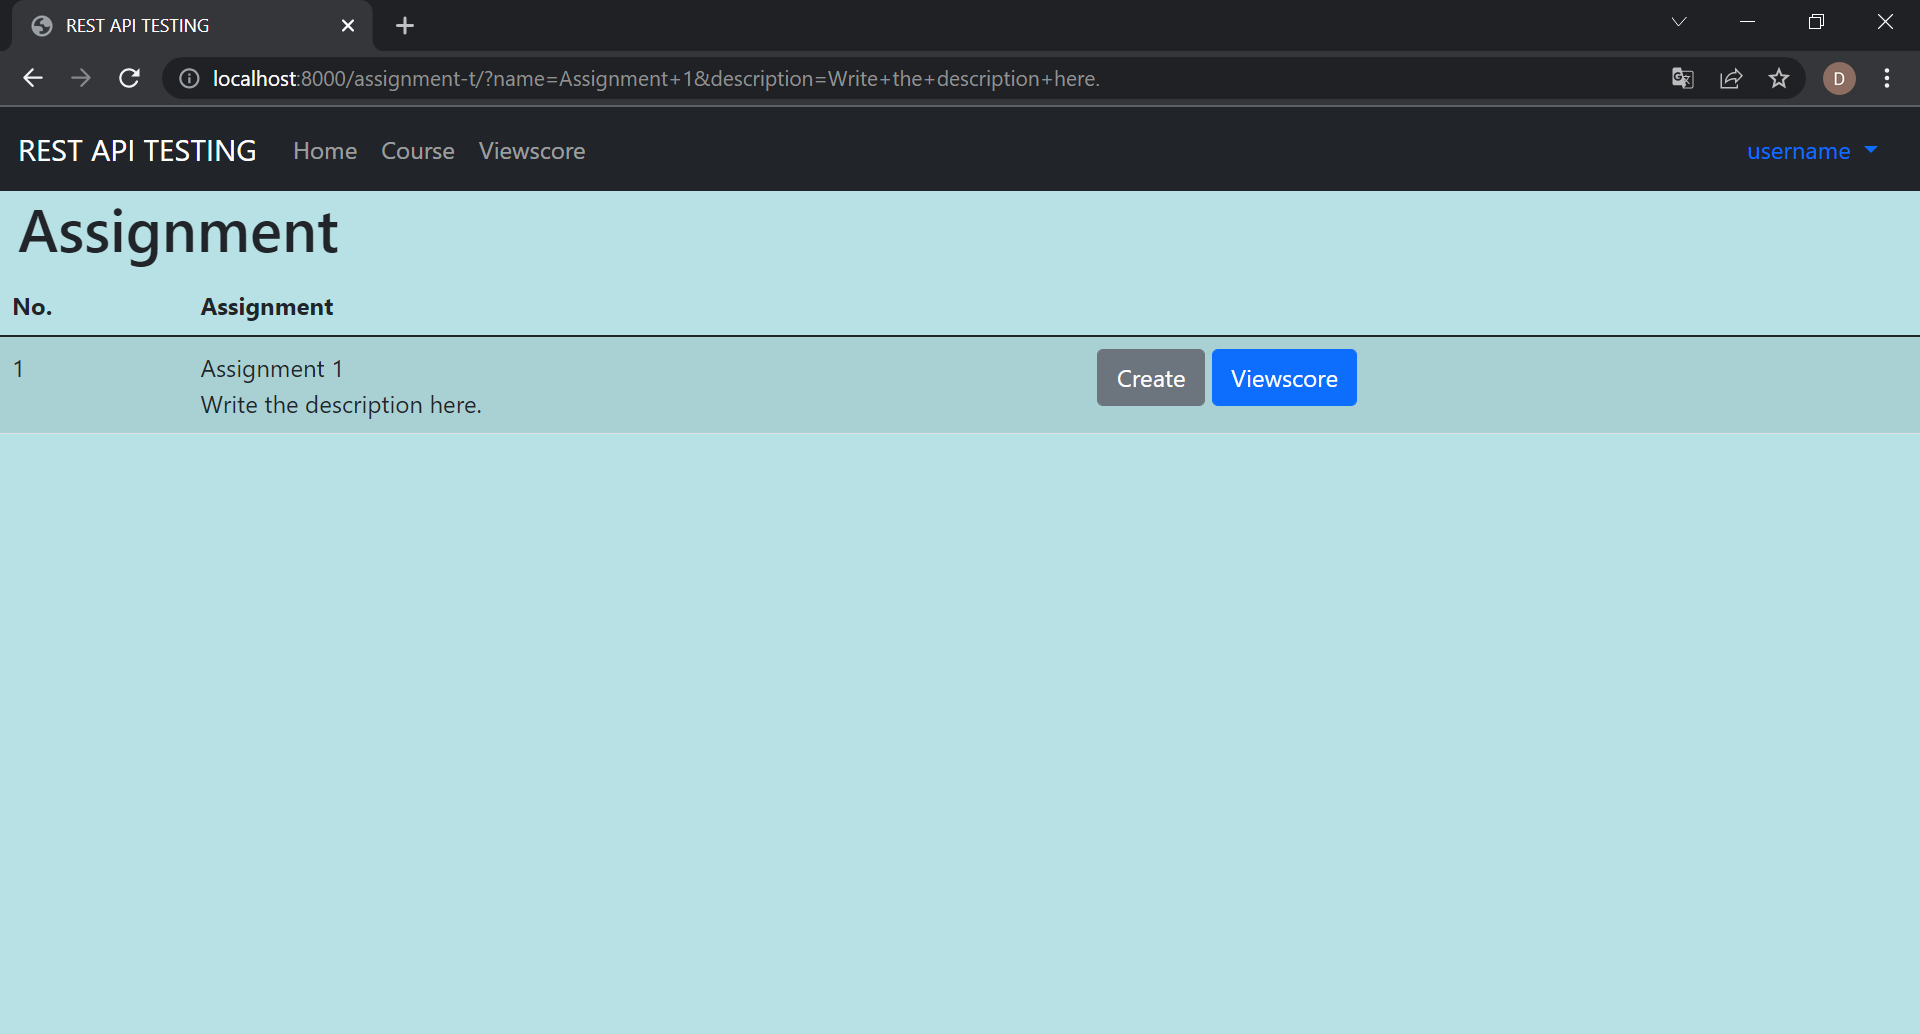
\includegraphics[width=5in]{figures/chapter4/assign1.PNG}
    \caption{แสดงรายชื่อ Assignment หลังจากสร้างเสร็จ}
    \label{figure:assign2}
\end{figure}
เมื่อทำการ Create Assignment เสร็จ จะเห็นชื่อ Assignment ที่เราทำการสร้างขึ้น พร้อมกับคำอธิบาย จากนั้นหาก Teacher ต้องการดูงาน และ คะแนนของ Student สามารถเข้าไปดูได้ที่หน้า Viewscore โดยการกดปุ่ม Viewscore ของ Assignment นั้น ๆ

\begin{figure}[H]
    \captionsetup{justification=centering}
    \centering
    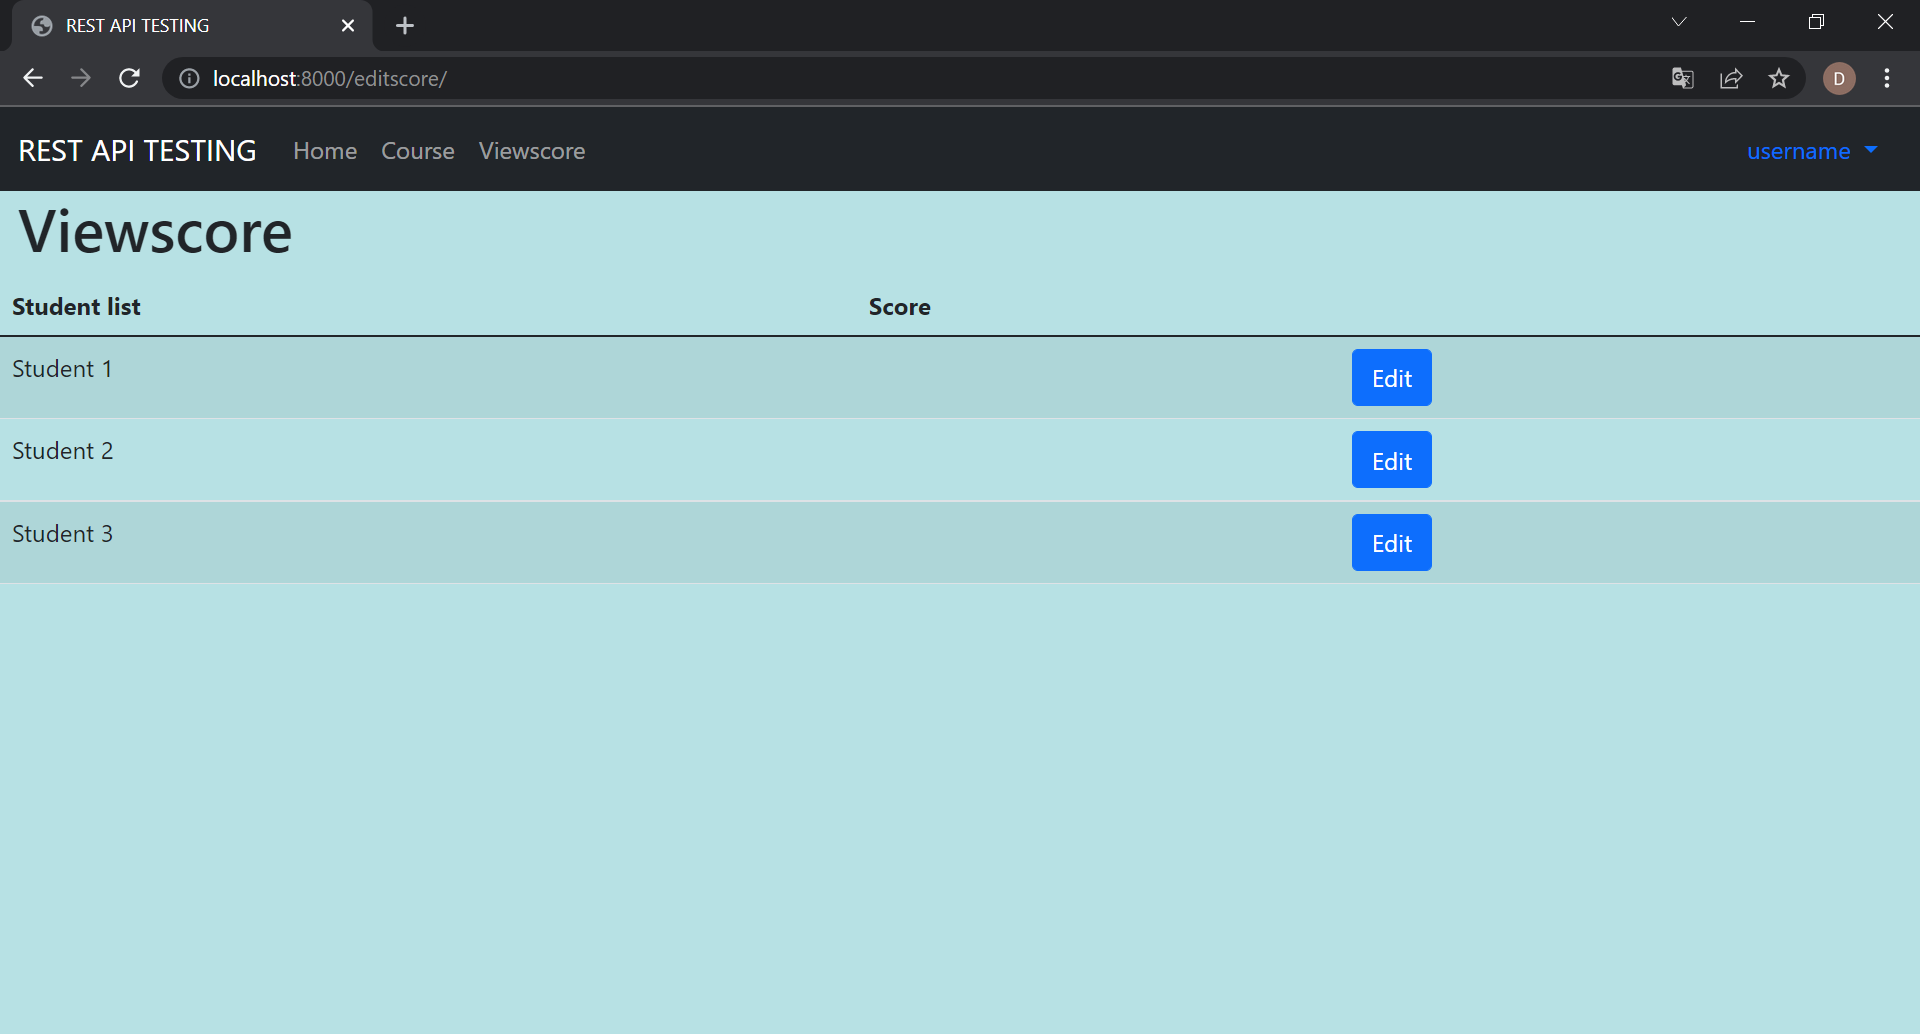
\includegraphics[width=5in]{figures/chapter4/editscore.PNG}
    \caption{หน้า Viewscore สำหรับดูคะแนน Student วิชานั้น}
    \label{figure:viewscore}
\end{figure}
เมื่อเข้ามายังหน้า Viewscore แล้ว Teacher จะสามารถเห็นรายชื่อ Student และ ไฟล์งานที่ Student ได้ทำการ Submit เข้ามา นอกจากนี้ยังสามารถดูคะแนนของ Student และ สามารถแก้ไขคะแนนได้จากปุ่ม Edit
\newpage

\subsection{ส่วนของ Student หรือ นักศึกษา}

\begin{figure}[H]
    \captionsetup{justification=centering}
    \centering
    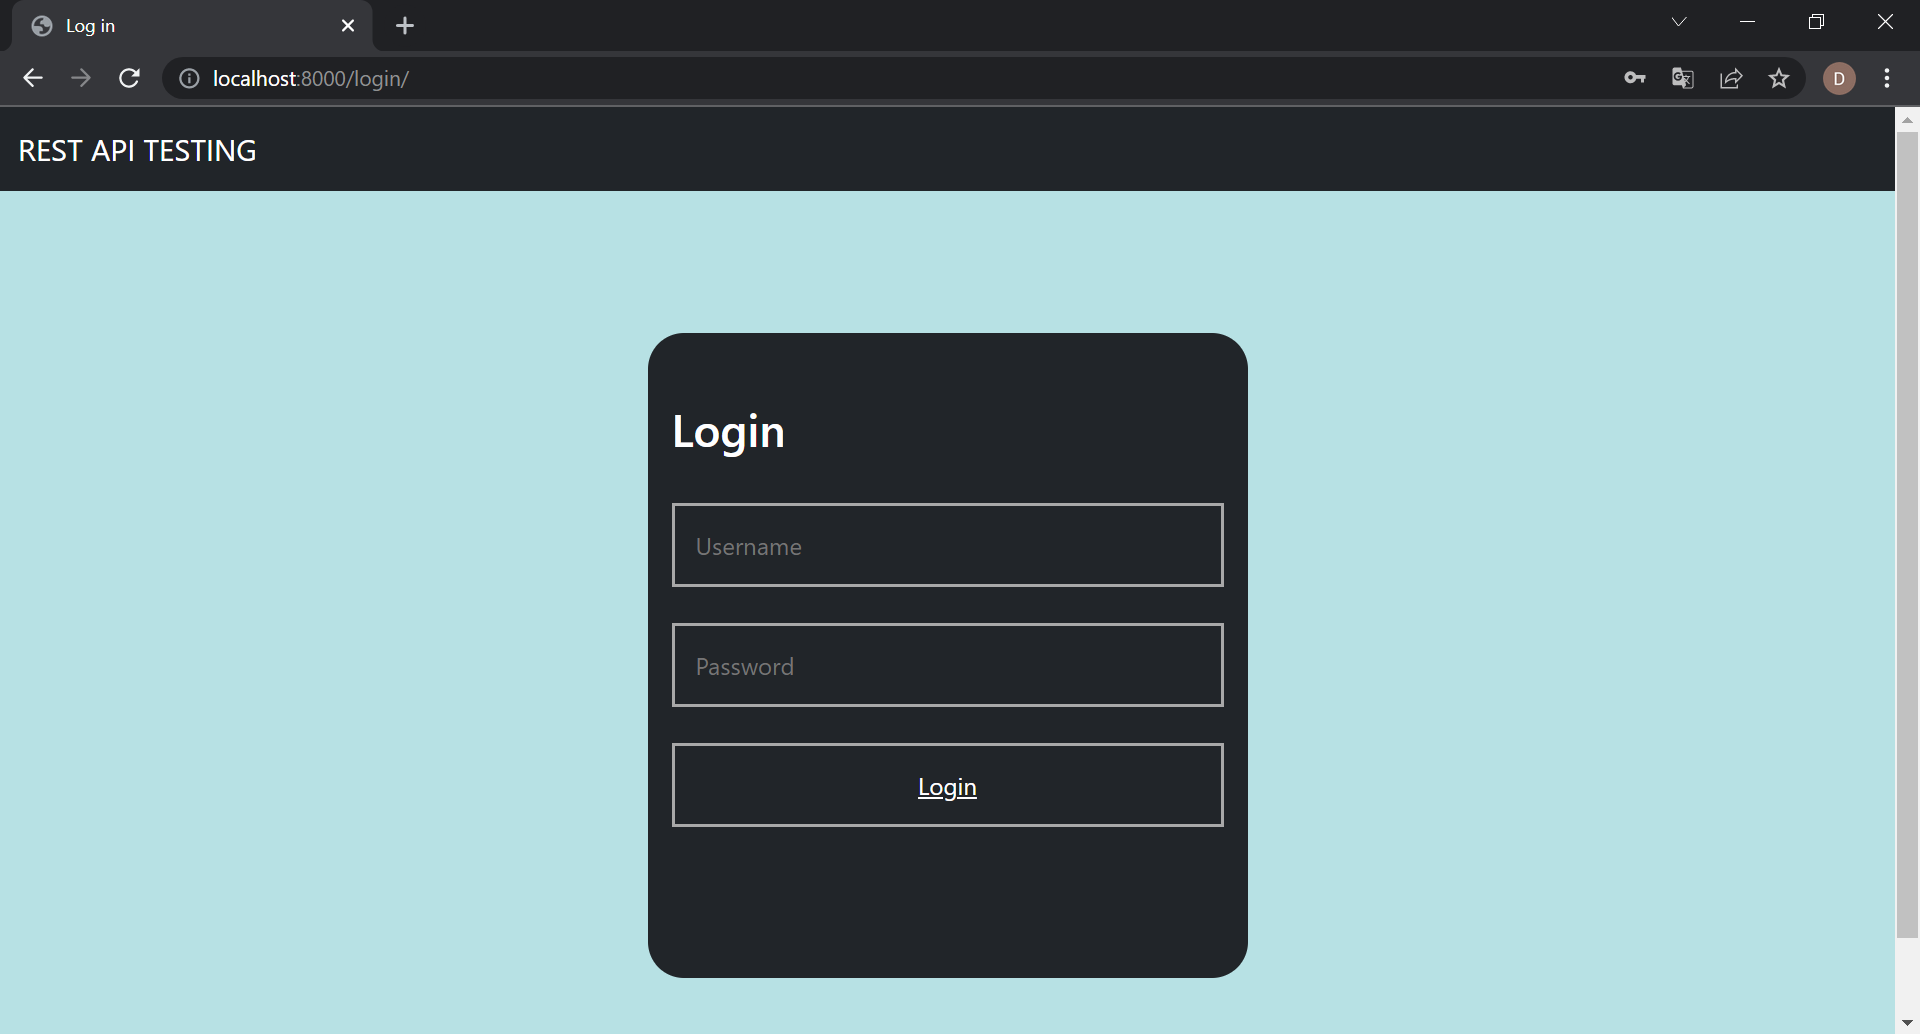
\includegraphics[width=5in]{figures/chapter4/login.PNG}
    \caption{หน้า Log in ฝั่ง Student}
    \label{figure:login2}
\end{figure}
Student ทำการ Log in ด้วย Username และ Password ของตนเองที่ถูกกำหนดสิทธิไว้่ให้สามารถเข้าถึงได้แค่บางส่วนที่จำเป็นเท่านั้นของหน้า Website ซึ่งหลังจากทำการ Log in เรียบร้อยแล้ว จะเข้ามายังหน้าของ Homepage ซึ่งเป็นหน้าแรกหลังจากทำการ Log in เรียบร้อยแล้ว

\begin{figure}[H]
    \captionsetup{justification=centering}
    \centering
    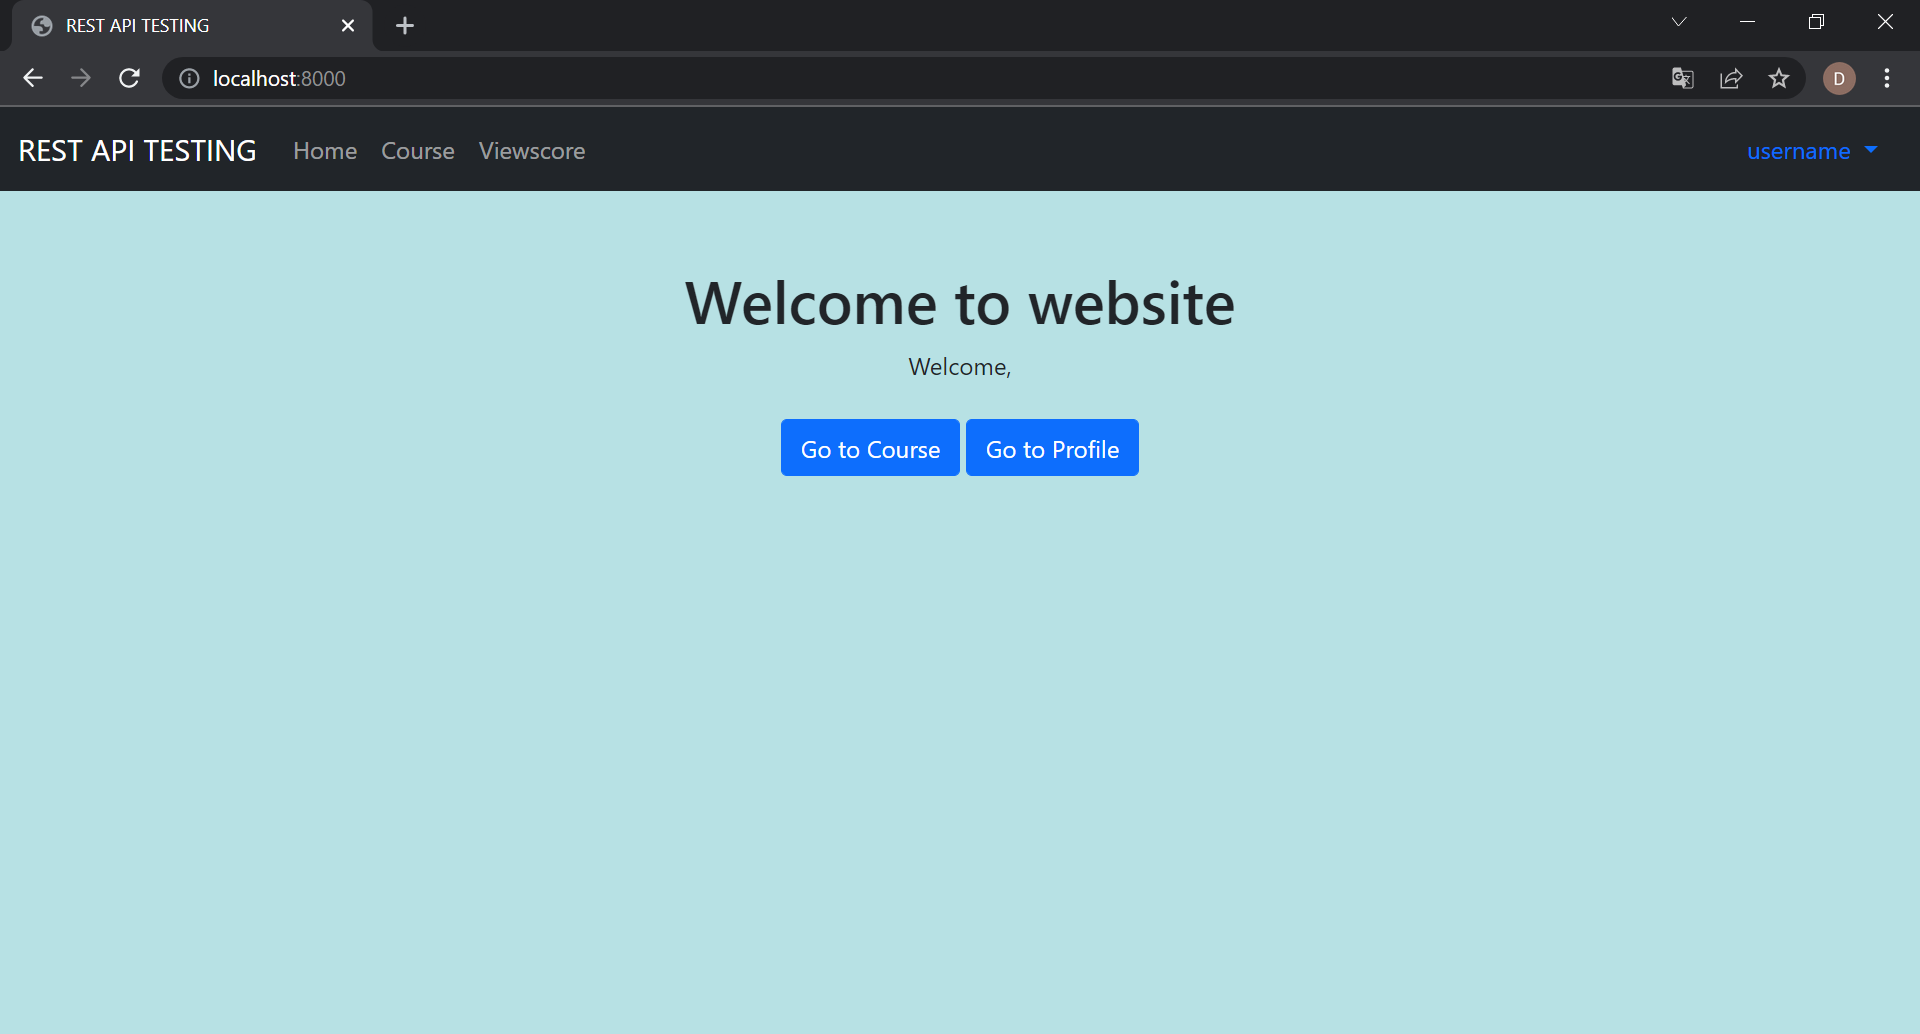
\includegraphics[width=5in]{figures/chapter4/homepage.PNG}
    \caption{หน้า Homepage ฝั่ง Student}
    \label{figure:homepage}
\end{figure}
เช่นเดียวกับ Teacher Student เมื่อเข้ามายังหน้า Homepage สามารถเข้าไปยังหน้าต่าง ๆ ของ Website ผ่านหน้าหลักนี้ ซึ่งจะแสดงเมนูต่าง ๆ ที่สามารถเข้าถึงได้ ซึ่งเมื่อกดปุ่ม Go to Course จะไปยังหน้า Course ที่แสดงวิชาเรียน และ เมื่อกดปุ่ม Go to Profile จะไปยังหน้า Profile
\newpage

\begin{figure}[H]
    \captionsetup{justification=centering}
    \centering
    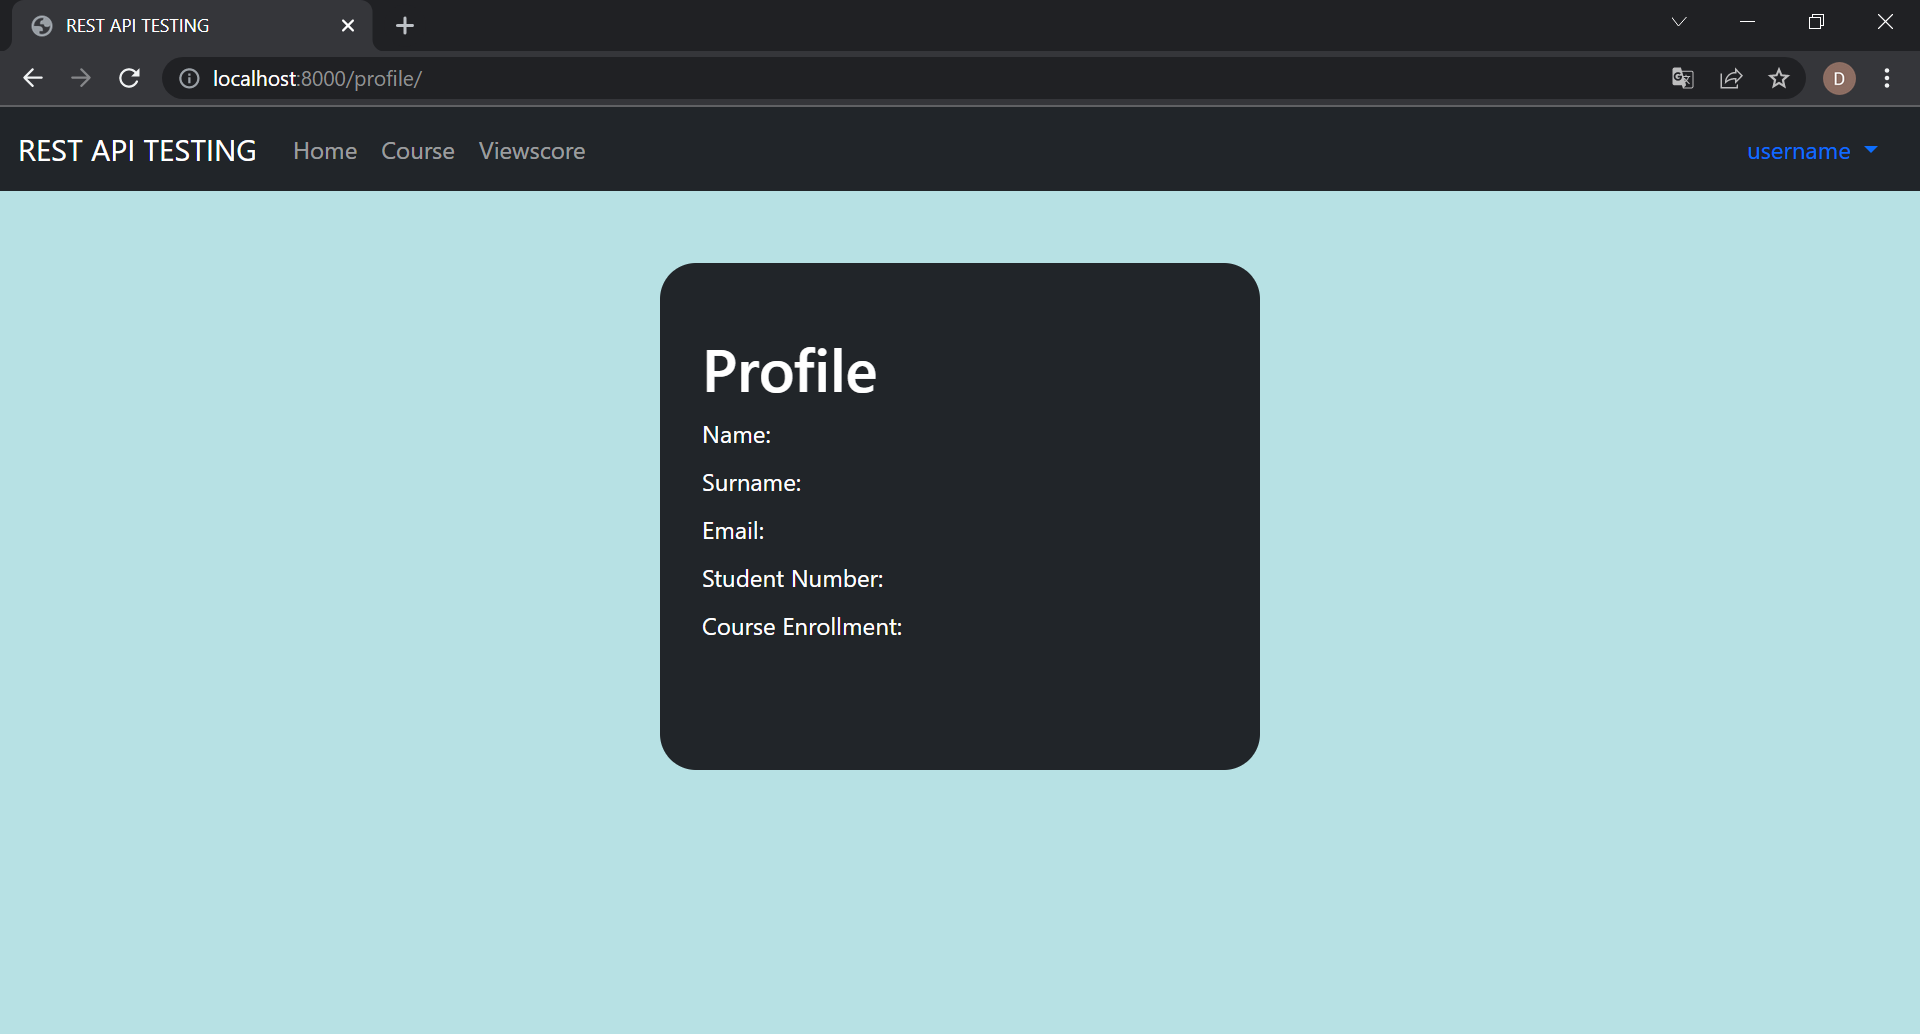
\includegraphics[width=5in]{figures/chapter4/profile.PNG}
    \caption{หน้า Profile ของ Student}
    \label{figure:profile}
\end{figure}
จากรูป \ref{figure:profile} เมื่อเข้ามาหน้า Profile แล้ว จะแสดงข้อมูลต่าง ๆ ของ Student

\begin{figure}[H]
    \captionsetup{justification=centering}
    \centering
    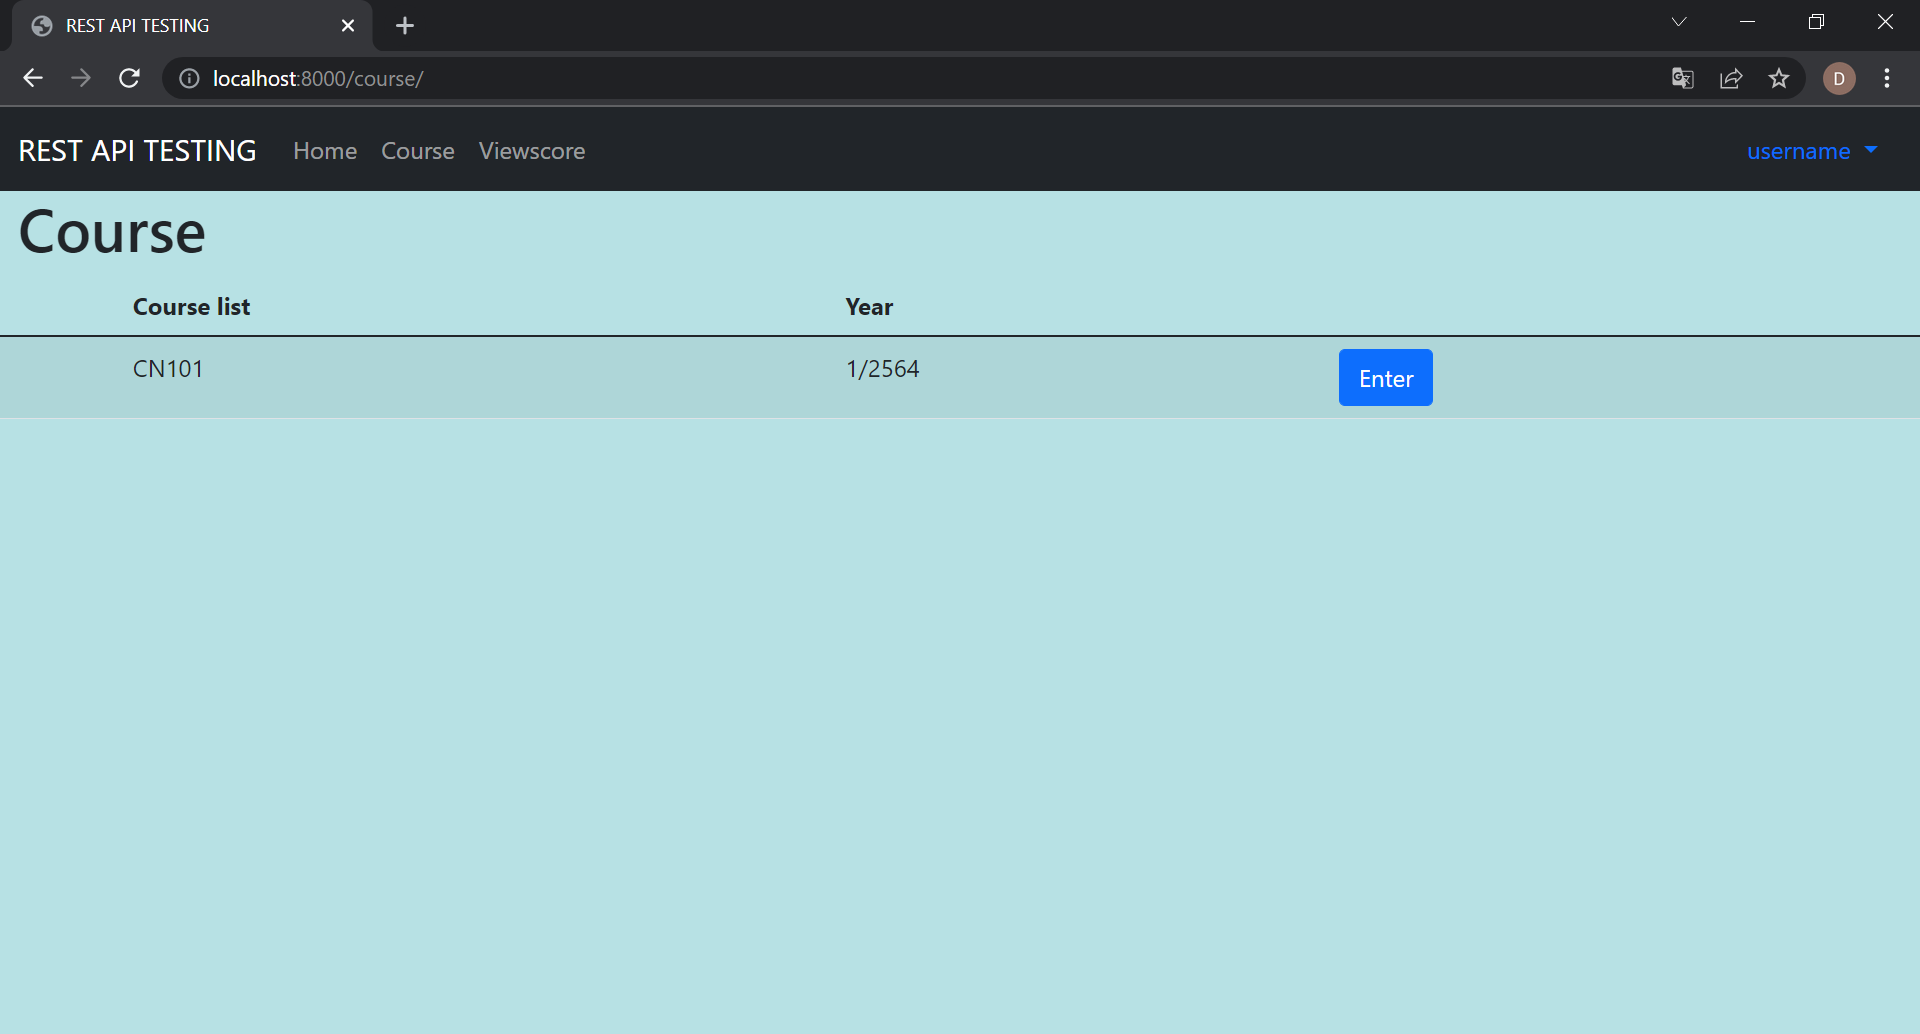
\includegraphics[width=5in]{figures/chapter4/coursestudent.PNG}
    \caption{แสดงรายวิชาฝั่ง Student}
    \label{figure:course3}
\end{figure}
จากรูป \ref{figure:course3} เมื่อเข้ามายังหน้า Course ของ Student จะแสดงวิชาเรียนต่าง ๆ ขึ้นมา เมื่อกด Enter จะสามารถเข้าไปยังหน้า Assignment ของ วิชานั้นได้
\newpage

\begin{figure}[H]
    \captionsetup{justification=centering}
    \centering
    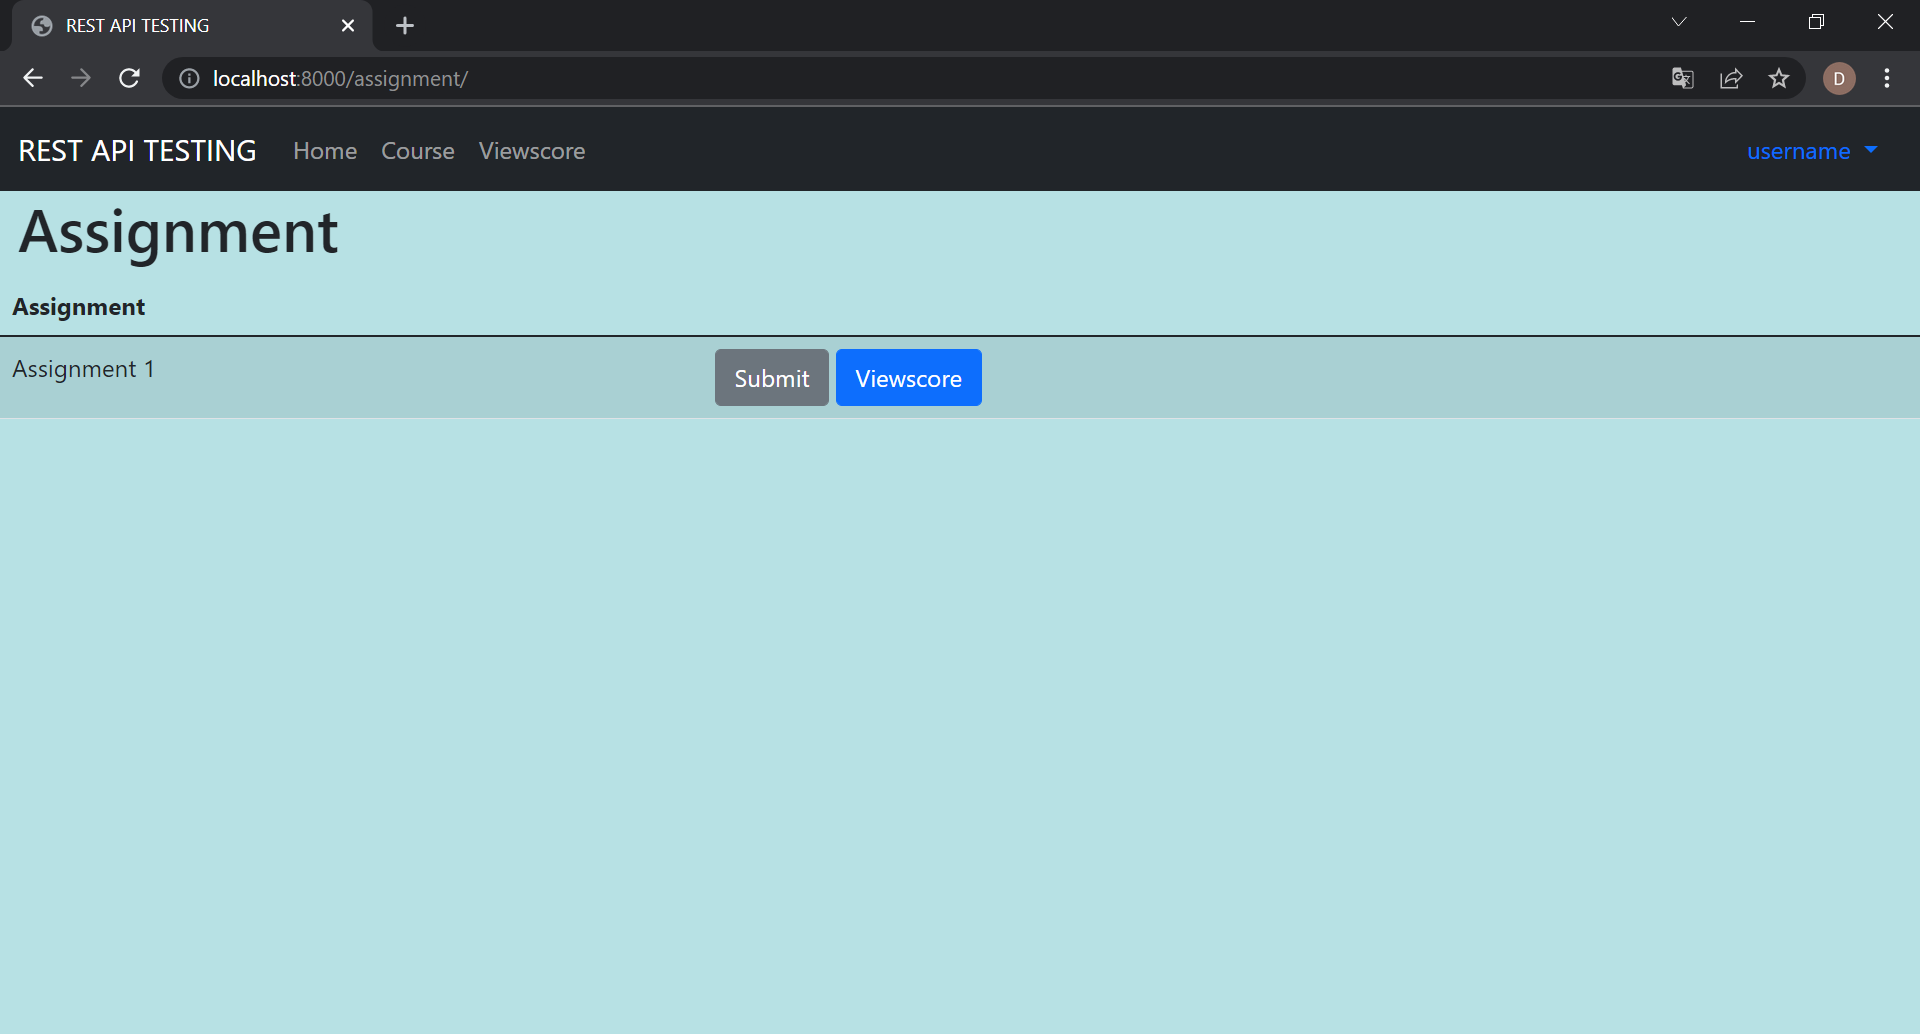
\includegraphics[width=5in]{figures/chapter4/assignstudent.PNG}
    \caption{แสดง Assignment ฝั่ง Student}
    \label{figure:assignment}
\end{figure}
เมื่อเข้ามายังหน้า Assignment แล้ว Student จะเห็น list ของ Assignment ที่ Teacher ได้ทำการสร้างไว้ เมื่อ Student ต้องการจะส่งงานของ Assignment นี้ ให้ทำการกด Submit จะสามารถ Upload ไฟล์งานลงไปได้ จากนั้น Student สามารถดูคะแนนของตนเองได้โดยการกดปุ่ม Viewscore เพื่อไปยังหน้า Viewscore เพื่อดูคะแนน

\begin{figure}[H]
    \captionsetup{justification=centering}
    \centering
    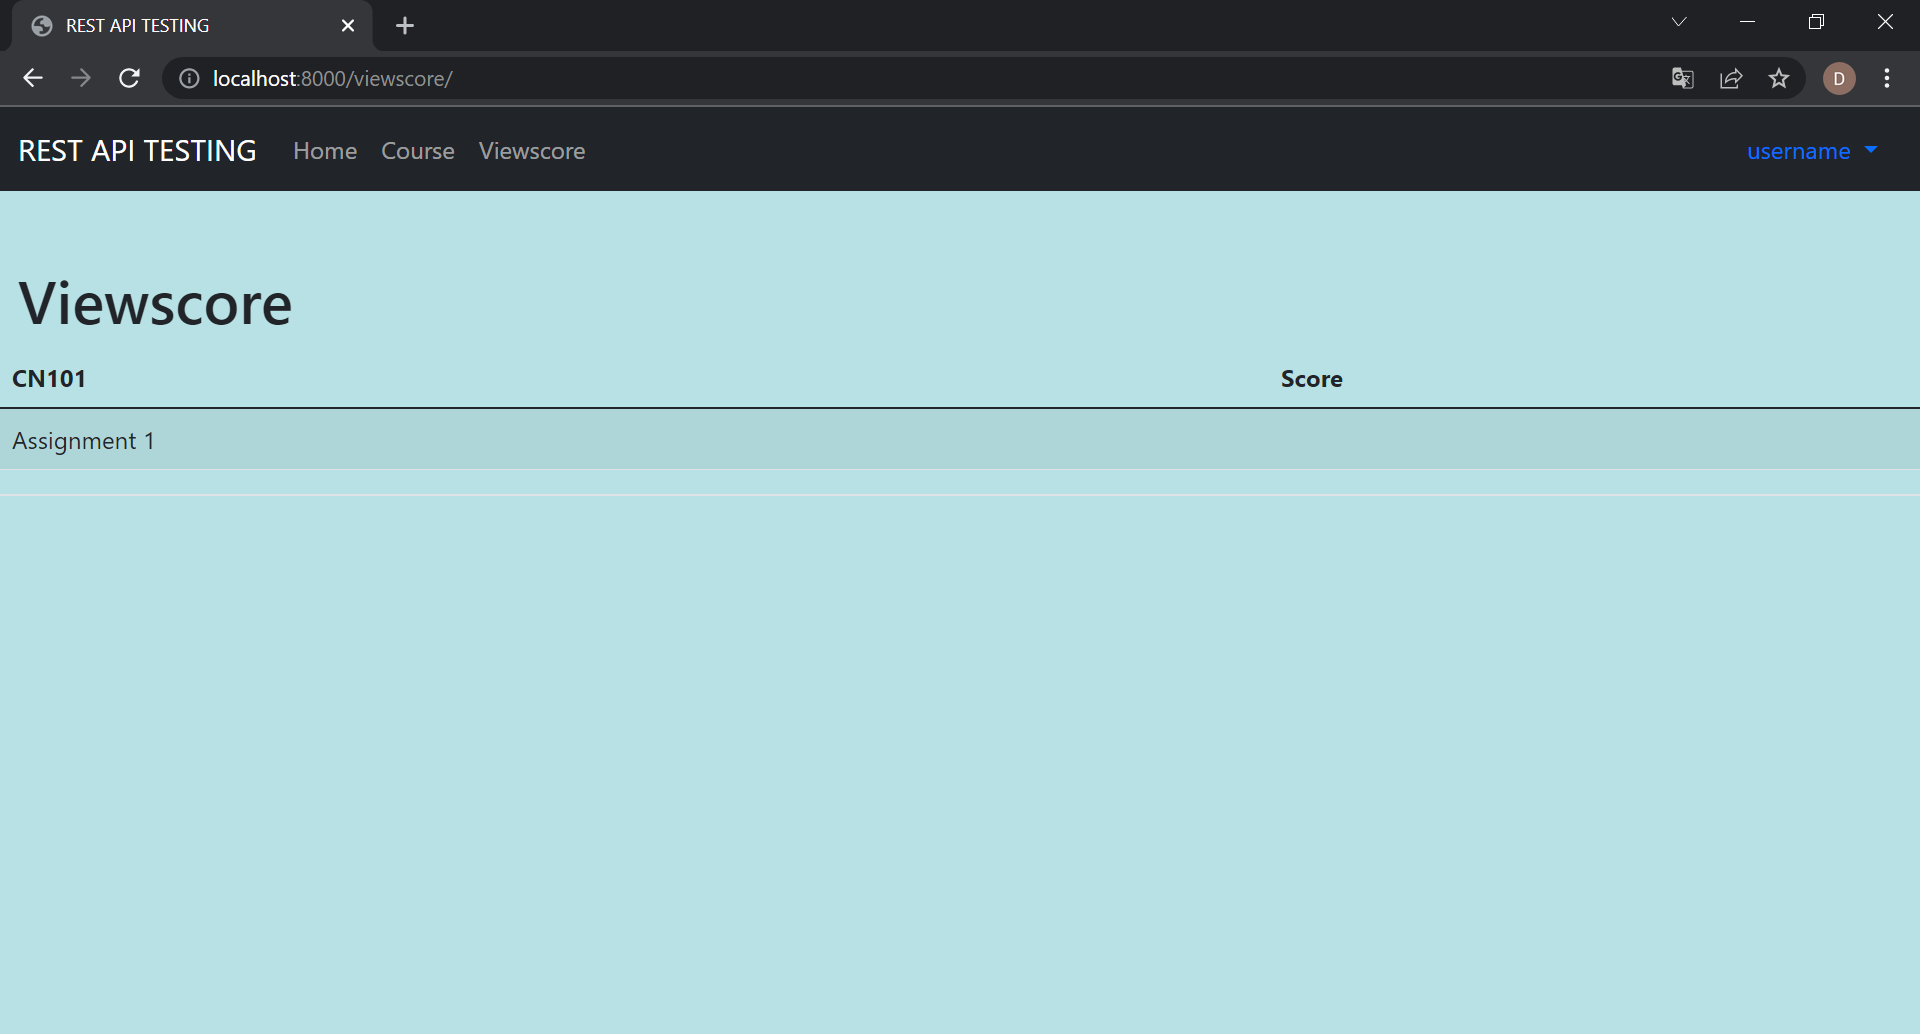
\includegraphics[width=5in]{figures/chapter4/viewscore.PNG}
    \caption{แสดงคะแนนของ Student แต่ละ Assignment ในวิชานั้น}
    \label{figure:score}
\end{figure}
จากรูป \ref{figure:score} จะแสดง Assignment ต่าง ๆ และ คะแนนที่ Student ได้รับ

